%\listfiles
\documentclass[11pt]{article}
\usepackage{fullpage}
%\usepackage{epsfig}
\usepackage{amssymb}
%\usepackage{a4}
\usepackage{fancyhdr}
\usepackage{subfigure}
\usepackage{ifthen}
\usepackage{version}
\usepackage{tocbibind}
\usepackage{makeidx}
%\usepackage{times}
\usepackage{booktabs}
\usepackage[colorlinks=true, pdfstartview=FitV, linkcolor=blue, 
            citecolor=blue, urlcolor=blue]{hyperref}
\usepackage{url}
\raggedbottom
\sloppy

\parindent=0pt
\parskip=5pt

\def\Dendroscope{{\sf Dendroscope }}

\newcommand{\out}[1]{}

%\newcommand\expert[1]{#1}   % expert mode on
\newcommand\expert[1]{}    % expert mode off

\newcommand{\cs}[1]{\textcolor{red}{#1}}



%%%%%%%%%%%%%%%%%%%%%%%%%%%%%%%%%%%%%%%%%%%%%%%
\input versioninfo.tex
%%%%%%%%%%%%%%%%%%%%%%%%%%%%%%%%%%%%%%%%%%%%%%%

%%%%%%%%%%%%%%%%%%%%%%%%%%%%%%%%%%%%%%%%%%%%%%%
\title{User Manual for \Dendroscope V\VERSION}
%%%%%%%%%%%%%%%%%%%%%%%%%%%%%%%%%%%%%%%%%%%%%%%

%%%%%%%%%%%%%%%%%%%%%%%%%%%%%%%%%%%%%%%%%%%%%%%

\author{Daniel H.~Huson and Celine Scornavacca}

%%%%%%%%%%%%%%%%%%%%%%%%%%%%%%%%%%%%%%%%%%%%%%%

\makeindex

\input definitions.tex

\ifx\pdfoutput\undefined
\usepackage[dvips]{graphicx}
\else
\usepackage[pdftex]{graphicx}
\fi

%%%%%%%%%%%%%%%%%%%%%%%%%%%%%%%%%%%%%%%%%%%%%%%
\begin{document}
%%%%%%%%%%%%%%%%%%%%%%%%%%%%%%%%%%%%%%%%%%%%%%%

\maketitle

\begin{center}

\includegraphics[width=0.7\textwidth]{./figs/about}
\end{center}

\tableofcontents

%%%%%%%%%%%%%%%%%%%%%%%%%%%%%%%%%%%%%%%%%%%%%%%
\mysection{Introduction}
%%%%%%%%%%%%%%%%%%%%%%%%%%%%%%%%%%%%%%%%%%%%%%%


\ibf{License}:
Copyright (c) 2015, Daniel H. Huson, with some code written by other authors, as mentioned in the corresponding source files.

This program is free software: you can redistribute it and/or modify
it under the terms of the GNU General Public License as published by
the Free Software Foundation, either version 3 of the License, or
(at your option) any later version.

This program is distributed in the hope that it will be useful,
but WITHOUT ANY WARRANTY; without even the implied warranty of
MERCHANTABILITY or FITNESS FOR A PARTICULAR PURPOSE.  See the
GNU General Public License for more details.

You should have received a copy of the GNU General Public License
along with this program.  If not, see \url{http://www.gnu.org/licenses}.

\ibf{Type-setting conventions}:
In this manual we use e.g.\ {\tt Edit}$\to${\tt Find} to indicate
the {\tt Find} menu item in the {\tt Edit} menu.

\ibf{How to cite}:
If you publish results obtained in part by using \Dendroscope, then we
require that you acknowledge this by \pwindow{citing the program} as follows:
\begin{itemize}
\item Daniel H. Huson and Celine Scornavacca. Dendroscope 3: An interactive tool for rooted phylogenetic trees and networks,
Systematic Biology (2012), \url{http://sysbio.oxfordjournals.org/cgi/content/abstract/sys062? ijkey=ZCxPRbYt74aQJhR&keytype=ref},
software freely available from
\href{http://www.dendroscope.org}{www.dendroscope.org}.
\end{itemize}

This manual is based on the user manual for Dendroscope~1, which was written by
Daniel H.~Huson, Daniel C.~Richter, Christian Rausch and Regula Rupp.

%%%%%%%%%%%%%%%%%%%%%%%%%%%%%%%%%%%%%%%%%%%%%%%
\mysection{Program Overview} 
%%%%%%%%%%%%%%%%%%%%%%%%%%%%%%%%%%%%%%%%%%%%%%%
\Dendroscope is a platform-independent software written in Java that enables conveniently to 
browse phylogenetic trees  and networks with up to hundreds of thousands of taxa.
Here is an overview of its features:
\begin{itemize}
\item There are 8 different tree views available, e.g. phylogram, cladogram or radial views.
\item Its novel navigational features facilitate the analysis of large trees.
\item It provides several tree manipulating functions like 
rerooting, subtree rotating, tree flipping and formatting features like renaming,
coloring or resizing edges, nodes and labels. 
\item A comprehensive set of export formats for the generation of images is available.
\item User formatted trees can be saved as a NeXML project file or as \textit{.nexus}, or Newick tree files. 
\item Tree structures (single or multiple) can be loaded from  \textit{.tre} (Newick format) or \textit{.nexus} files or entered manually.
\item Rooted phylogenetic networks can be entered and visualized using the \concept{Extended Newick} format \cite{Cardona2008}.
\item 
The program permits the computation of consensus trees  from a set of input trees.
\item The program also permits  the computation of rooted phylogenetic networks (among others cluster networks \cite{ClusterNetworks2008}, {galled networks} \cite{GalledNetworks2009}, {minimum networks} \cite{LevelKClusters2010} and hybridization networks  \cite{Albrecht2012,HusonLinz2012}) from a set of input trees.
\item It provides several tree manipulating functions like 
rerooting, subtree rotating, tree flipping and formatting features like renaming,
coloring or resizing edges, nodes and labels. 


\end{itemize}

%%%%%%%%%%%%%%%%%%%%%%%%%%%%%%%%%%%%%%%%%%%%%%%
\mysection{Obtaining and Installing the Program}
%%%%%%%%%%%%%%%%%%%%%%%%%%%%%%%%%%%%%%%%%%%%%%%
\Dendroscope is written in Java and requires a Java runtime environment
version 1.7 or later, freely available from
\href{http://www.java.org}{www.java.org}. %\marginpar{CS: v 1.6?}

\Dendroscope is installed using an installer program that is freely available
from\\
\href{http://www.dendroscope.org}
{www.dendroscope.org}.
There are three different installers, targeting different operating systems:
\begin{itemize}
\item \itt{Dendroscope\_windows\_\VERSION.exe} provides an installer for \irm{Windows}.
\item \itt{Dendroscope\_macos\_\VERSION.dmg} provides an installer for \irm{MacOS}.
\item \itt{Dendroscope\_unix\_\VERSION.sh} provides a shell installer for
\irm{Linux} and \irm{Unix}.
\end{itemize}

Alternatively \Dendroscope will be available as Java \pwindow{Webstart application} from \\
\href{http://ab.inf.uni-tuebingen.de/data/software/dendroscope/webstart/}{http://ab.inf.uni-tuebingen.de/data/software/dendroscope/webstart/}.
If you need information concerning Java Webstart, go to \href{http://java.sun.com/products/javawebstart/}{http://java.sun.com/products/javawebstart/}.


%\pagebreak
%%%%%%%%%%%%%%%%%%%%%%%%%%%%%%%%%%%%%%%%%%%%%%%
\mysection{Getting Started}
%%%%%%%%%%%%%%%%%%%%%%%%%%%%%%%%%%%%%%%%%%%%%%%
This section describes how to get started and to do the first steps of analyses 
using \Dendroscope.

First, download an installer for the program from 
\href{http://www.dendroscope.org}
{www.dendroscope.org},
see Section~\ref{sec:Obtaining and Installing the Program}
for details.

Start the program and load any \textit{.tre}, \textit{.nexus}, \textit{.nexml} or \textit{.dendro} 
project file via \menuitem{File}{Open}. Alternatively, if the file
was recently opened by the program, then it may be contained in
the \menuitem{File}{Open Recent} submenu.\\
At startup, the tree will be scaled to fit to the window size. 

Draw the tree differently by choosing one of the 8 provided views e.g. 
\menuitem{Layout}{Draw Rectangular Phylogram},
\menuitem{Layout}{Draw Rectangular Cladogram},
\menuitem{Layout}{Draw Slanted Cladogram},
\menuitem{Layout}{Draw Circular Phylogram},
\menuitem{Layout}{Draw Circular Cladogram},
\menuitem{Layout}{Draw Inner Circular Cladogram},
\menuitem{Layout}{Draw Radial Phylogram},
\menuitem{Layout}{Draw Radial Cladogram}.
Try out the magnifier functions by clicking on \menuitem{View}{Use Magnifier}.
Change any label font, size, color or edge/node size/width by opening the  \window{Format Panel}
via \menuitem{Edit}{Format}.

If you want to print the current image
choose \menuitem{File}{Print}. In case you need a quality image of the tree, simply export it to several 
file formats via \menuitem{File}{Export Image}.

Finally, if you want to save the tree(s) and the formatting click \menuitem{File}{Save As} generating a \textit{.nexml} project file.
You can also export the tree(s) by clicking \menuitem{File}{Export}. Choose one of the export formats (newick or nexus).

Note that only by saving a formatted tree as a \textit{.nexml} project file
you can save the formatting with the tree.

%%%%%%%%%%%%%%%%%%%%%%%%%%%%%%%%%%%%%%%%%%%%%%%
\mysection{Main Window}
%%%%%%%%%%%%%%%%%%%%%%%%%%%%%%%%%%%%%%%%%%%%%%%
The \pwindow{Main} window is used to display the taxonomy and to
control the program via the main menus.

We now discuss all menus of the \window{Main} window. 

%%%%%%%%%%%%%%%%%%%%%%%%%%%%%%%%%%%%%%%%%%%%%%%
\mysubsection{File Menu}
The \pmenu{File} menu contains the following file-related items:
\begin{itemize}
\item The \pmenuitem{File}{New} item opens a new document. Any selected trees are put in it.
\item The \pmenuitem{File}{Open} item provides an \pwindow{Open File} dialog
to open one or more files containing input data. The supported formats are 
\textit{.nexml}, \textit{.dendro}, \textit{.tre}, \textit{.nexus} (see Section \ref{dendroscopefileformat}).
Note that the standard open dialog does not allow one to open more than one file under MacOS X.
As a work-around, press the shift-key when selecting the  \menuitem{File}{Open}  menu item so as to obtain
an alternative file open dialog that allows one to select more than one file for opening.
\item The \pmenuitem{File}{Open Recent} can be used to re-open a recently opened file.
\item The \pmenuitem{File}{Add From File} item adds trees or networks from a file to the current document.
\item The \pmenuitem{File}{Enter Trees or Networks} item enters trees in Newick or networks in extended Newick format.
\item The \pmenuitem{File}{Save} item saves the current document in NeXML format.
\item The \pmenuitem{File}{Save As} item saves the current document under a new name.
\item The \pmenuitem{File}{Export} item 
opens the \pwindow{Choose output format} dialog
which is used to export the current trees or networks in a number of file 
formats, see  Section \ref{dendroscopefileformat}. 
\item The \pmenuitem{File}{Duplicate} item duplicates this document.
\item The \pmenuitem{File}{Export Image} item  opens the \window{Export Image} dialog
which is used to save the current network in a number of different graphics
formats, see Section~\ref{subsec:Graphics Formats}.
\item The \pmenuitem{File}{Page Setup} item setups the page for printing.
\item The \pmenuitem{File}{Print} item prints the network.
\item The \pmenuitem{File}{Close} item closes the current window. In case only one window is opened, the application exits.
\item The \pmenuitem{File}{Quit} item quits the program (Windows and Linux only).
\end{itemize}   


%%%%%%%%%%%%%%%%%%%%%%%%%%%%%%%%%%%%%%%%%%%%%%%
\mysubsection{Edit Menu}
The \pmenu{Edit} menu contains the usual edit-related items:
%\marginpar{\cs{?}} %\cs{check swap etc, only when panel is on}
\begin{itemize}
\item The \pmenuitem{Edit}{Copy} item is used to copy the current tree or network or all selected trees or networks.
\item The \pmenuitem{Edit}{Copy Image} item is used to copy the current tree or network or all selected trees or networks as an image that can be pasted into another program, e.g. PowerPoint.
\item The \pmenuitem{Edit}{Paste} item is used to paste the copied trees or networks to a new tab.
\item The \pmenuitem{Edit}{Find} item opens the
\window{Find} tool bar which can be used to search for taxa.
\item The \pmenuitem{Edit}{Find Again} item finds the next occurrence of a search
string.
\item The \pmenuitem{Edit}{Replace} item opens the
\window{Replace} tool bar which can be used to replace taxon names.
\item The \pmenuitem{Edit}{Reroot} item reroots the tree or the network at the specified nodes or edge. If more than node is selected, all selected taxon labels
are intepreted as\pconcept{outgroup} taxa and the program
determines the ``tightest'' rooting so that the outgroup appear
together below the root. If several nodes share the same label, all these nodes are considered to determine the ``tightest'' rooting. 
\item The \pmenuitem{Edit}{Swap Subtrees} item swaps the order of subtrees (or subnetworks) below the specified node (or nodes).
%,see also Section \ref{subsec:Navigating trees with keys and mouse wheel}\marginpar{\cs{?}}.%\cs{check the subsec:Navigating}
\item The \pmenuitem{Edit}{Rotate Subtrees} item rotates the order of the subtrees (or subnetworks) below the specified node(s).
\item The \pmenuitem{Edit}{Reorder Subtrees} item
opens  the \pwindow{Reorder subtrees} dialog that allows one to specific any type of reordering
of the children of the specified node using ``drag and drop'.%\marginpar{\cs{?}}.  %\cs{It should be only for one node}
\item The \pmenuitem{Edit}{Delete Taxa} item removes the selected taxa in the selected trees or networks%\marginpar{\cs{?}}. %\cs{work for newtorks?}
\item The \pmenuitem{Edit}{Unlock Edge Lengths}  item is used to ``unlock edge lengths'' so that
the user is allowed to reshape trees or networks by dragging nodes or internal edge points.

\item The \pmenuitem{Edit}{Format} item opens a \window{Format Panel} which provides several 
possibilities to change color, fonts, node and edge shapes and the positioning of the labels of the tree.
\end{itemize}

%%%%%%%%%%%%%%%%%%%%%%%%%%%%%%%%%%%%%%%%%%%%%%%
\mysubsection{Select Menu}
The \pmenu{Select} menu contains items for selecting panels and different sets
of substructures of trees or networks.
\begin{itemize}	
\item The \pmenuitem{Select}{Advanced Selection} submenu contains a number of advanced selection menu items that are probably
not of general interest.
\item The \pmenuitem{Select}{All Panels} item selects all panels.
\item The \pmenuitem{Select}{No Panels} item deselects all panels.
\item The \pmenuitem{Select}{Invert Panels} item inverts the selection of all panels.
\item The \pmenuitem{Select}{Select All} item is used to select all nodes and edges.
\item The \pmenuitem{Select}{Select Nodes} item is used to select all nodes.
\item The \pmenuitem{Select}{Select Edges} item is used to select all edges.
\item The \pmenuitem{Select}{From Previous Window} item is used to apply the selection of the previous window to the active window.
\item The \pmenuitem{Select}{Deselect All} item is used to deselect all nodes and edges that are currently selected.
\item The \pmenuitem{Select}{Deselect Nodes} item is used to deselect all nodes that are currently selected.
\item The \pmenuitem{Select}{Deselect Edges} item is used to deselect all edges that are currently selected.
\item The \pmenuitem{Select}{Select Labeled Nodes} item is used to select all labeled nodes.
\item The \pmenuitem{Select}{Select Leaves} item is used to select all leaves.
\item The \pmenuitem{Select}{Select Root} item is used to select the root node of the tree.
\item The \pmenuitem{Select}{Select Non-Terminal} item is used to select all non-terminal
nodes and edges.
\item The \pmenuitem{Select}{Select Special} item is used to select all edges leading to reticulation nodes in networks.
\item The \pmenuitem{Select}{Invert Selection} item is used to invert the current selection.
\item The \pmenuitem{Select}{Scroll to Selection} item is used to scroll to the current selection.
\item The \pmenuitem{Select}{List Selected Taxa} item is used to list all selected taxa.
\end{itemize}

{\small
The advanced selection submenu contains the following items:
\begin{itemize}
\item The \pmenuitem{Advanced Selection}{Select Subnetwork} item is used to select the subtree or subnetwork below a selected inner node or edge..
\item The \pmenuitem{Advanced Selection}{Select Induced Network} item is used to select a subtree or subnetwork induced by the set of currently selected nodes.
\item The \pmenuitem{Advanced Selection}{Select LSA Induced Network} item is used to select the  subtree or subnetwork rooted at  the LSA of the selected nodes.
\item The \pmenuitem{Advanced Selection}{Select Spanned Edges} item is used to select all edges spanned by the set of currently selected nodes.%\marginpar{\cs{?}}.%working for networks?
\end{itemize}
}

%%%%%%%%%%%%%%%%%%%%%%%%%%%%%%%%%%%%%%%%%%%%%%%

\mysubsection{Options Menu}
The \pmenu{Options} menu contains items for collapsing nodes and extracting subtrees.
\begin{itemize}
\item The \pmenuitem{Options}{Advanced Options} submenu contains some advanced options that are probably not
of general interest.
\item The \pmenuitem{Options}{Collapse} item enables to collapse subtrees or subnetworks below the  specified nodes. The former subtrees or subnetworks  are replaced by rectangles.
\item The \pmenuitem{Options}{Uncollapse} item is used to uncollapse (expand) the selected, collapsed subtrees or  subnetworks .
\item The \pmenuitem{Options}{Uncollapse Subtree} item is used to uncollapse (expand) all collapsed subtrees or subnetworks below  the  specified nodes.
\item The \pmenuitem{Options}{Collapse Complement} item is used to collapse all subtrees or  subnetworks except the currently selected part of the tree or  subnetwork%\marginpar{\cs{!}}.%not working 
\item The \pmenuitem{Options}{Collapse at Level} item is used to collapse all subtrees or  subnetworks at the specified level from the root. 
\item The \pmenuitem{Options}{Load Taxon Images} item is used to specify a directory containing
image files. Dendroscope tries to match taxon names to the names of images files and for each match
found, Dendroscope shows the image near the node representing the given taxon (recognized formats: GIF, JPG, JPEG, BMP and PNG). %\marginpar{\cs{!}}%not working in the new window
\item The \pmenuitem{Options}{Set Image Size} item is used to set the size of the image for the currently selected
nodes.
\item The \pmenuitem{Options}{Image Position} submenu is used to determine the relative positions of images
in relative to the corresponding nodes (North, South, East, West, Radial).%\marginpar{\cs{!}}%not working in the new window
\item The \pmenuitem{Options}{Next Tree} item moves to the next tree.
\item The \pmenuitem{Options}{Previous Tree} item moves to the previous tree.
\item The \pmenuitem{Options}{Go to Tree} item goes to a specific tree.
\item The \pmenuitem{Options}{Set Tree Name} item sets the name of a tree or network.
\end{itemize}

{\small
The advanced options submenu contains the following items:
\begin{itemize}
\item The \pmenuitem{Advanced Options}{Extract Subnetwork} item is used to extract a subtree or subnetwork below a node or edge.
\item The \pmenuitem{Advanced Options}{Extract Induced Network} item is used to extract a  subtree or subnetwork induced by the selected nodes to a new file.
\item The \pmenuitem{Advanced Options}{Extract LSA Induced Network} item is used to extract a  subtree or subnetwork rooted at the LSA of the selected nodes to a new file.
\item The \pmenuitem{Advanced Options}{Extract Induced Restriction} item is used to extract the restriction induced by the  selected nodes to a new file.
\end{itemize}
}

%%%%%%%%%%%%%%%%%%%%%%%%%%%%%%%%%%%%%%%%%%%%%%%

\mysubsection{Algorithms Menu}
The \pmenu{Algorithms} menu contains items for computing networks from trees and for comparing trees or networks.
\begin{itemize}
\item The \pmenuitem{Algorithms}{Advanced Algorithms} submenu contains additional advanced algorithms that are probably not
of general interest.
\item  The \pmenuitem{Algorithms}{Strict Consensus} item is used to compute the \pconcept{strict consensus} of a set of trees.
\item  The \pmenuitem{Algorithms}{Loose Consensus} item is used to compute the \pconcept{loose consensus} of a set of trees.
\item  The \pmenuitem{Algorithms}{Majority Consensus} item is used to compute the \pconcept{majority consensus} of a set of trees.
\item  The \pmenuitem{Algorithms}{LSA Consensus} item is used to compute the \pconcept{LSA consensus} of a set of trees \cite{PhylogeneticNetworks2010}.
\item  The \pmenuitem{Algorithms}{Primodial Consensus} item is used to compute the \pconcept{primodial consensus} of a set of trees \cite{Primodial2013}.
\item  The \pmenuitem{Algorithms}{Network Consensus}~item is used to compute a 
\pconcept{rooted network consensus} of a set of trees. 

If the input set contains more than two trees, then the user can set a 
threshold that determines the percentage of input trees that a cluster must be 
contained in to make it into the output rooted network.
The user can also 
decide whether the program should come a \pconcept{cluster network} 
\cite{ClusterNetworks2008} that shows the clusters in a
\pconcept{hardwired representation}, a
\pconcept{galled network} \cite{GalledNetworks2009} that represents the clusters in a 
topologically restricted \pconcept{softwired representation},
or a \pconcept{minimum network} that attempts to represent the
clusters in a network of minimum \pconcept{level},
as described in \cite{LevelKClusters2010}.
\item
The \pmenuitem{Algorithms}{Network for Multi-Labeled Tree} menu item is used to compute a rooted
phylogenetic network for a multi-labeled tree such that the network contains each label (or taxon)
exactly once. There are three methods available here: the \pconcept{cluster-based method}
extracts all the clusters in the tree and constructs a cluster network.
The \pconcept{exact method} computes the nested label for the root node of the tree and
then constructs the corresponding network for that label \cite{HOLM2007}.
The \pconcept{level-k-based} method extracts all clusters and then seeks to compute a level-$k$ network
of minimum level $k$ for the clusters.
\item The \pmenuitem{Algorithms}{Hybridization Network} item computes all minimum {hybridization networks} for two rooted
phylogenetic trees, not necessarily binary, on overlapping taxon sets using the Autumn algorithm \cite{HusonLinz2012}.
\item The \pmenuitem{Algorithms}{Hybridization Network (Binary Trees)} item computes all minimum {hybridization networks} for two bifurcating trees on the same taxon set  \cite{Albrecht2012}.
\item The \pmenuitem{Algorithms}{Reroot By Hybridization Number} item determines a rooting that minimizes the
hybridization number, given two rooted
phylogenetic trees, not necessarily binary, on overlapping taxon sets, using the Autumn algorithm \cite{HusonLinz2012}.
\\item The \pmenuitemh{Algorithms}{Tanglegram} item is used to compute a \pconcept{tanglegram} for two trees or networks using a NeighborNet-based heuristic \cite{Tanglegrams}.
\end{itemize}

Note that  Dendroscope does not require that the trees all contain exactly the same set of taxa to be able
to compute a consensus (unlike most other programs), as it uses
the Z-closure method to merge partial data \cite{zclosure}.%\marginpar{\cs{?}} %Z-closure?

{\small
The advanced algorithms submenu contains the following items:
\begin{itemize}
\item the \pmenuitem{Advanced Algorithms}{Hybridization Number} item is used to compute the {hybridization number} for two rooted trees using the Autumn algorithm \cite{HusonLinz2012}. Trees need not be binary and need not have identical taxon
sets.
\item the \pmenuitem{Advanced Algorithms}{Hybridization Number (Binary Trees)} item is used to compute the {hybridization number} for two selected rooted binary trees on the same taxon set \cite{Albrecht2012}.
\item the \pmenuitem{Advanced Algorithms}{rSPR Distance (Binary Trees)} item  is used to compute the {rSPR distance} for two selected rooted binary trees on the same taxon set \cite{whiddenWABI}.
\item the \pmenuitem{Advanced Algorithms}{DTL Reconciliation} item  is used to calculate the {DTL reconciliation} between two binary trees \cite{Doyon10}.
\item the \pmenuitem{Advanced Algorithms}{Hardwired Cluster Distance} item  is used to calculate the \emph{hardwired cluster distance} between two trees or networks \cite{PhylogeneticNetworks2010}.
\item the \pmenuitem{Advanced Algorithms}{Softwired Cluster Distance} item  is used to calculate the \emph{softwired cluster distance} between two trees or networks  \cite{PhylogeneticNetworks2010}.
\item the \pmenuitem{Advanced Algorithms}{Displayed Trees Distance} item  is used to calculate the \emph{displayed trees distance} between two trees or networks \cite{PhylogeneticNetworks2010}.
\item the \pmenuitem{Advanced Algorithms}{Tripartition Distance} item  is used to calculate the \emph{tripartition distance} between two trees or networks \cite{MNWRTPST2004}.
\item the \pmenuitem{Advanced Algorithms}{Nested Labels Distance} item  is used to calculate the \emph{nested labels distance} between two trees or networks \cite{CLRV2009d,Nakhleh2009}.
\item the \pmenuitem{Advanced Algorithms}{Path Multiplicity Distance} item  is used to calculate the \emph{path multiplicity distance} between two trees or networks \cite{CardonaTreeChildNetworks2008}.
\item The \pmenuitem{Advanced Algorithms}{Simplistic} item computes a phylogenetic networks using the \pconcept{simplistic algorithm} \cite{VanIersel2009}.
\end{itemize}
}

%%%%%%%%%%%%%%%%%%%%%%%%%%%%%%%%%%%%%%%%%%%%%%%
\mysubsection{Layout Menu}
The \pmenu{Layout} menu contains items for different tree and network views \cite{Huson2009}.
\begin{itemize}
\item The \pmenuitem{Layout}{Draw Rectangular Phylogram} item is used to draw  trees or networks  as rectangular phylograms.
\item The \pmenuitem{Layout}{Draw Rectangular Cladogram} item is used to draw trees or networks as rectangular cladograms.
\item The \pmenuitem{Layout}{Draw Slanted Cladogram} item is used to draw trees or networks as slanted cladograms.
\item The \pmenuitem{Layout}{Draw Circular Phylogram} item is used to drawtrees or networks as circular phylograms.
\item The \pmenuitem{Layout}{Draw Circular Cladogram} item is used to draw  as circular cladograms.
\item The \pmenuitem{Layout}{Draw Inner Circular Cladogram} item is used to draw trees or networks as circular cladograms with leaves on the inside.
\item The \pmenuitem{Layout}{Draw Radial Phylogram} item is used to draw trees or networks as radial phylograms.
\item The \pmenuitem{Layout}{Draw Radial Cladogram} item is used to draw trees or networks as radial cladograms.
\item The \pmenuitem{Layout}{Ladderize Left} item is used to order trees or networks so that the largest clades appear leftmost (uppermost in the view).
\item The \pmenuitem{Layout}{Ladderize Right} item is used to order trees or networks so that the largest clades appear rightmost (lowermost in the view).
\item The \pmenuitem{Layout}{Ladderize Random} item is used to order the clades randomly.
\item The \pmenuitem{Layout}{Network Layout} item is used to choose the way the network embedding is computed. There are four methods available here. With \pconcept{No Optimization}, we do not attempt to optimize the embedding of networks. The \pconcept{2008 Algorithm} optimizes embedding of networks using the algorithm
described in (Kloepper and Huson 2008). The \pconcept{2009 Algorithm} optimizes embedding of networks using the algorithm
described in (Huson 2009). The \pconcept{2010 Algorithm} optimizes embedding of networks using a new algorithm
developed by Huson and Scornavacca in 2010.

\item The \pmenuitem{Layout}{Align Taxa} item: Attempts to align taxa in all selected trees or networks
using an algorithm described in \cite{Tanglegrams}.
\item The \pmenuitem{Layout}{Connect Taxa} item: Connect all taxa of the same name in different trees or networks.
\item The \pmenuitem{Layout}{Disconnect All} item: Disconnect all nodes in different trees or networks.
\end{itemize}
%%%%%%%%%%%%%%%%%%%%%%%%%%%%%%%%%%%%%%%%%%%%%%%

%%%%%%%%%%%%%%%%%%%%%%%%%%%%%%%%%%%%%%%%%%%%%%%
\mysubsection{View Menu}
\label{views}
The \pmenu{Views} menu contains items for setting the grid, scaling trees or networks, using the magnifier and showing/hiding labels.
\begin{itemize}
\item The \pmenuitem{View}{Set Grid} item is used to set  the tree or network grid dimensions.
\item The \pmenuitem{View}{Less Panels} item is used to lessen the number of panels in the grid.
\item The \pmenuitem{View}{More Panels} item is used to increase the number of panels in the grid.
\item The \pmenuitem{View}{Show Scroll Bars} item is used to show or hide scroll bars.
\item The \pmenuitem{View}{Show Borders} item is used to show or hide borders.
\item The \pmenuitem{View}{Show Scale Bar} item is used to show or hide scale bar.
\item The \pmenuitem{View}{Zoom to Fit} item is used to scale the tree or network to fit the window.
\item The \pmenuitem{View}{Fully Contract} item is used to contract the tree or network.
\item The \pmenuitem{View}{Fully Expand} item is used to expand the whole tree or network.
\item The \pmenuitem{View}{Use Magnifier} item is used to turn the
\concept{magnifier functionality}  on and off.
\item The \pmenuitem{View}{Magnify All Mode} item modifiers the magnification process
so that the whole tree gets mapped into the magnifier.
\item The \pmenuitem{View}{Show Node Labels} item is used to make all node labels visible or invisible.
\item The \pmenuitem{View}{Show Edge Labels} item is used to make \irm{edge labels} visible or invisible.
\item The \pmenuitem{View}{Label Edges By Weights} item uses the edge weights as edge labels.
\item The \pmenuitem{View}{Sparse Labels} item instructs the program to show only a subset of the taxon labels, thus avoiding overlapping labels.
\item The \pmenuitem{View}{Radial Labels} item instructs the program to rotate leaf labels
to match the orientation of the edges that lead to them.
\item The \pmenuitem{View}{Reposition Labels} item sets all the labels to their original position.
\end{itemize}


%%%%%%%%%%%%%%%%%%%%%%%%%%%%%%%%%%%%%%%%%%%%%%%
\mysubsection{Window Menu}
The \pmenu{Window} menu contains a number of window-related commands
as well as a list of all currently open windows.
\begin{itemize}
\item The \pmenuitem{Window}{About} item opens a splash screen showing the program version. In MacOS, this can be found under \pmenuitem{Dendroscope}{About}.
\item The \pmenuitem{Window}{How to Cite} item shows the citation info for this software which is:\\
(1) Daniel H Huson, Daniel C Richter, Christian Rausch, Tobias Dezulian, Markus Franz and Regula Rupp. Dendroscope: An interactive viewer for large phylogenetic trees . BMC Bioinformatics 8:460, 2007. (2) Daniel H Huson and Celine Scornavacca.  Dendroscope 3: a tool for drawing, modifying and computing rooted phylogenetic networks. In preparation.
	\item The \pmenuitem{Window}{Website} item is used to go to the program website.
\item The \pmenuitem{Window}{Set Window Size} item is used to set the
size of the \window{Main} window.
\item The \pmenuitem{Window}{Command-line Syntax} item lists all commands supported by the program.
\item The \pmenuitem{Window}{Command Input} item opens a window that can be used to enter a command (see \concept{command}).
%\item The \pmenuitem{Window}{Add Tree or Network} item opens a window to enter
tree or network manually in Newick Format. 
\item The \pmenuitem{Window}{Message Window} item is used to open the \window{Message} window.
\item If several program windows are opened, they are listed at the end of the window menu.
\end{itemize}

%%%%%%%%%%%%%%%%%%%%%%%%%%%%%%%%%%%%%%%%%%%%%%%
\mysubsection{Toolbar}
For easier access of frequently used functions, a \pconcept{Toolbar} is provided.
The button images are self-explicative and a description appears when passing on the buttons with the mouse.

%%%%%%%%%%%%%%%%%%%%%%%%%%%%%%%%%%%%%%%%%%%%%%%
\mysubsection{Context Menus}

A right mouse click when the index finger of the hand icon is positioned on a node opens a context menu which allows to
edit the node label, open the \window{Format Panel}, show or hide node labels, copy the node label, select the subtree starting from this node, and swap the subtree starting from this node.

A right mouse click when the index finger of the hand icon is positioned on an edge opens a context menu which allows to
edit the edge label, open the \window{Format Panel}, show or hide edge labels, and copy the edge label.

A right mouse click beside the tree opens a context menu which allows to select or deselect all edges, nodes, and labels, to scale the tree or network to fit the window or finally to show or hide scroll bars and borders.



%%%%%%%%%%%%%%%%%%%%%%%%%%%%%%%%%%%%%%%%%%%%%%%
\mysubsection{Status Line}
The \pwindow{Status Line} at the bottom of the program window shows the index of the current tree,
the total number of trees, the number of nodes and edges and the available space of the reserved memory. 


%%%%%%%%%%%%%%%%%%%%%%%%%%%%%%%%%%%%%%%%%%%%%%%
\mysection{Additional Windows}


%%%%%%%%%%%%%%%%%%%%%%%%%%%%%%%%%%%%%%%%%%%%%%%
\mysubsection{Format Panel}
The \pwindow{Format Panel} can be opened via \menuitem{Edit}{Format} or by a right mouse click 
after selecting elements of the tree like edges, nodes or labels.
You can format them as follows:

\begin{itemize}
\item Edges can have their \irm{edge width} and  \irm{edge width}  set.
\item Edges can be assigned three types of shapes: \irm{straight edges}, \irm{curved edges}
and \irm{angular edges},
the effect of which depends on the current view.
\item Nodes can be assigned certain shapes: \irm{square nodes}, \irm{circle nodes} or none.
Square and circle \irm{node shapes} can have their \irm{node size} and \irm{node color} set.
\item 
If a selected node or edge has a label, then you can choose its \irm{font family}, \irm{font style}
or \irm{font size}.
\item Labels can be switched on and off, and can be rotated to the left or right. \index{show/hide labels}
\index{rotate labels}
\end{itemize}

Configuration changes are applied immediately.
The \pmenuitem{Options}{Save Font As Default} menu item
can be used to set the default font, style and size used by the program. \index{default font, setting}

%%%%%%%%%%%%%%%%%%%%%%%%%%%%%%%%%%%%%%%%%%%%%%%
\mysubsection{Find and Replace Toolbars}

The \pwindow{Find} toolbar can be opened or closed using the
\menuitem{Edit}{Find} menu item. Its purpose is to search  labels
in the displayed trees or networks. Enter a query specifying the text to find
 in the top text region.
Use the following check boxes to configure the search:
\begin{itemize}
\item If the \pbutton{Case sensitive} item is selected, then the case of
letters is distinguished in comparisons.
\item If the \pbutton{Whole words only} item is selected, then only taxa or labels
matching the complete query string will be returned.
\item If the \pbutton{Regular Expression} item is selected,
the query is interpreted as a Java regular expression (see example further down).
\end{itemize}

The scope of the search can be \itt{Global} or \itt{Selection}.
If a searched label is "hidden" inside a bounding box (black opaque area of tree or network) or in a collapsed branch,
it will be selected.

Press the \itt{Close}, \itt{Find First},  \itt{Find Next} or \itt{Find All}
buttons to close the toolbar, or find the first, or next occurrence
of the query, respectively. Press \itt{Unselect All} to unselect the highlighted  occurrences.

The \pwindow{Replace} toolbar can be opened or closed using the
\menuitem{Edit}{Replace}  menu item. Its purpose is to replace  text
in the displayed trees or networks. Enter a replacement text in the bottom text region.

Press the \itt{Replace} or  \itt{Replace All} buttons to replace the next or all occurrences
of the query with the  text in the bottom text region, respectively. 

\ignore{
Alternatively, it is possible to provide Dendroscope with a query file: use the \itt{From File} 
 button to find all nodes that
match any line of the  input file. The \button{Case sensitive} , \button{Whole words only} 
and \button{Regular Expression} buttons
apply to this type of search, too. \index{finding taxa from a file} .
}

\textbf{Regular Expressions} are powerful and flexible text-processing tools.
They allow to specify complex patterns of text that can be discovered in an input string.

{\bf Example 1:}

Each of the following represent valid regular expressions, and all will successfully
match the character sequence "\texttt{Escherichia}":
\begin{itemize}
\item Escherichia
\item E.*
\item \lbrack eE\rbrack scherichia
\item \lbrack eE\rbrack sch\lbrack aeiou\rbrack \lbrack a-z\rbrack ichi.*
\end{itemize}

{\bf Example 2:}

To select the five taxa simultaneously, e.g.\ Human, Mouse, Dog, Cat and Rat,
use the following expression: {\tt Human|Mouse|Dog|cat|Rat} and then press \pbutton{Find All}.

For an extensive list of metacharacters and further explanations go to http://java.sun.com/j2se/1.5.0/docs/api/java/util/regex/Pattern.html



%%%%%%%%%%%%%%%%%%%%%%%%%%%%%%%%%%%%%%%%%%%%%%%
\mysubsection{Message Window}
The \pwindow{Message} window is opened using the
\menuitem{Window}{Message Window} item.
The program writes all internal messages to this window.
The window contains the usual File and Edit menu items.

%%%%%%%%%%%%%%%%%%%%%%%%%%%%%%%%%%%%%%%%%%%%%%%
\mysubsection{Export Image Dialog} \label{openexportimagedialog}
The \pwindow{Export Image} dialog is opened using the
\menuitem{File}{Export Image} item.
This dialog is used to save an image of the current tree
in a number of different formats, see Section~\ref{subsec:Graphics Formats}. 

The dialog permits to specify the file name and  where to save the graphics file.
The format is chosen from a menu.
There are two radio buttons \pbutton{Save whole image}
to save the whole image, and \pbutton{Save visible region} to save
only the part of the image that is currently visible in the main viewer.
%If the chosen format is \pwindow{EPS}, then selecting
%the \pbutton{Convert text to graphics} check box will request the program
%to render all text as graphics, rather than fonts.


%%%%%%%%%%%%%%%%%%%%%%%%%%%%%%%%%%%%%%%%%%%%%%%
\mysubsection{About Window}
The \pwindow{About} Window is opened using the
\menuitem{Window}{About} submenu (\menuitem{Dendroscope}{About} in MacOS). It reports the version of the program and its authors.
%%%%%%%%%%%%%%%%%%%%%%%%%%%%%%%%%%%%%%%%%%%%%%%

%here today

%%%%%%%%%%%%%%%%%%%%%%%%%%%%%%%%%%%%%%%%%%%%%%%
\mysection{Additional Features}

%%%%%%%%%%%%%%%%%%%%%%%%%%%%%%%%%%%%%%%%%%%%%%%
\mysubsection{Using the Mouse to Select}

Nodes, edges and labels can also be selected by clicking on them with the index finger of the hand icon\index{click selection}.
If the left  mouse click is press for 2 seconds or shift-clicking\index{shift-click selection}, an arrow appears:
dragging the mouse\index{selection}, it is possible to perform a  \irm{rubber-band selection} in which all objects contained within a dragged rectangle
are selected.

%%%%%%%%%%%%%%%%%%%%%%%%%%%%%%%%%%%%%%%%%%%%%%%
\mysubsection{Magnifier Functionality}
Dendroscope provides the user with a \pconcept{magnifier functionality} that can be used to
magnify portions of the tree.

Selecting the \menuitem{View}{Use Magnifier} item adds a magnifier layer to the view.
\begin{itemize}
\item {\em Magnifier band}:
For all rooted views (rectangular and slanted view) a \pconcept{magnifier band} is laid over the tree. 
\item {\em Magnifier disk}:
For all unrooted views (radial and circular tree view) a \pconcept{circular} magnifier is 
laid over the tree.
\end{itemize}

The magnifier can be pulled to a desired position by grabbing its frame with the mouse.
The radius/width of the magnifier can be changed by dragging the rhomb at the magnifier's border line.
The zoom factor of the magnifier can be changed via the [+,-] button.\\
Two magnifier modes are available depending on the current tree view.

%%%%%%%%%%%%%%%%%%%%%%%%%%%%%%%%%%%%%%%%%%%%%%%

\mysubsection{Navigating trees with keys and mouse wheel}
%%%%%%%%%%%%%%%%%%%%%%%%%%%%%%%%%%%%%%%%%%%%%%%

 \Dendroscope allows one to browse and analyze trees.
\pwindow{Navigating trees} is facilitated by some \pwindow{key bindings}:
\begin{itemize}
\item {\em Scrolling:} 
Hold down the Shift button and use the mouse wheel to scroll top-down.\\
Hold down the Alt and Shift buttons and use the mouse wheel to scroll right-left.
\item {\em Zooming:} 
Use the mouse wheel to zoom the tree. Zooming is centered on the current mouse position.
Press the shift key to zoom the graph in 
horizontal direction. 
\item {\em Rotating:} 
For circular and radial drawings, use the shift-key and
left and right arrow keys to rotate the tree.
\end{itemize}

Alternatively, use the arrow keys to scroll the tree or network, or
additionally press the shift key to zoom the graph in 
horizontal or vertical direction (zoom not available in this way for  circular and radial drawings). Use the alt and control keys
for acceleration.


%%%%%%%%%%%%%%%%%%%%%%%%%%%%%%%%%%%%%%%%%%%%%%%
\mysection{File Formats}\label{dendroscopefileformat}
%%%%%%%%%%%%%%%%%%%%%%%%%%%%%%%%%%%%%%%%%%%%%%%
\Dendroscope uses the NeXML   file format to store the data of the modified 
and/or formatted tree or network.
By convention, we use the suffix \textit{.nexml} 
for NeXML files.


%%%%%%%%%%%%%%%%%%%%%%%%%%%%%%%%%%%%%%%%%%%%%%%
\mysubsection{NeXML files}
Dendroscope saves trees 
in a simple text-based format with the file extension \texttt{.nexml}. It contains the tree in Newick notation and additional (machine-readable) information on the view, selections, coloring etc. of the saved trees.	%\marginpar{\cs{!}} %check this

Trees can also be saved in Nexus and Newick format. However, when these formats are used, all information on the layout of the trees, fonts, colors, line widths etc are lost.

%%%%%%%%%%%%%%%%%%%%%%%%%%%%%%%%%%%%%%%%%%%%%%%

\mysubsection{Old Dendroscope files}

For backward compatibility, this version of Dendroscope can still open  \texttt{.dendro} files (see the old version of this manual).

%%%%%%%%%%%%%%%%%%%%%%%%%%%%%%%%%%%%%%%%%%%%%%%
\mysubsection{Nexus files}
Dendroscope can read a Nexus file that contains a \irm{Nexus trees block} and can export trees in this format.

%%%%%%%%%%%%%%%%%%%%%%%%%%%%%%%%%%%%%%%%%%%%%%%
\mysubsection{Newick files}
Dendroscope can read Newick files and can export trees in this format.

%%%%%%%%%%%%%%%%%%%%%%%%%%%%%%%%%%%%%%%%%%%%%%%

%%%%%%%%%%%%%%%%%%%%%%%%%%%%%%%%%%%%%%%%%%%%%%%
\mysubsection{Extended Newick format and rooted phylogenetic networks}

The \pconcept{Extended Newick} format was designed as an extension of the Newick format
to be able to describe rooted phylogenetic networks in bracket notation.
Unfortunately, there is not just one such format, but a number of different ones.
Dendroscope implements a version of the Extended-Newick proposed by \cite{Cardona2008}.% \marginpar{\cs{!}} %check this
%format that arose out of discussions
%that took place
%during the Phylogenetics Programme at the Isaac Newton Institute in 2007.

In Dendroscope, a rooted phylogenetic network is described as a single line of extended-Newick format using brackets, as in the
description of a rooted phylogenetic tree in the standard Newick format, with additional
labels placed at the end of node labels. These special labels are of the form
'\#H1', '\#H2', etc. When parsing an extended-Newick string, all nodes whose labels end on '\#H1' are identified
with each other, all nodes that end on '\#H2' are identified, etc.

For example, to describe a rooted phylogenetic network with three leaves labeled 'a', 'b' and 'c',
in which 'b' is to have a ``reticulate'' parent node that connects both above 'a' and above 'c',
use the following extended-Newick string:
\begin{verbatim}
((a,(b)#H1),(c,#H1));
\end{verbatim}
Copy and paste this string into a Dendroscope window to see the corresponding network.

In Dendroscope, quite everything that can be done with a rooted tree can also be done with a rooted phylogenetic network!

%%%%%%%%%%%%%%%%%%%%%%%%%%%%%%%%%%%%%%%%%%%%%%%
\mysubsection{Graphics Formats}
The following \pwindow{graphics formats} are supported (how to open the \texttt{Export Image} dialog see \ref{openexportimagedialog}):

\begin{itemize}
\item \irm{JPEG}, ``Joint Photographic Experts Group''.
\item \irm{GIF}, ``Graphics Interchange Format''.
%\item \irm{EPS}, ``Encapsulated PostScript''. \marginpar{\cs{?}} %not working
\item \irm{SVG}, ``Scalable Vector Graphics''.
\item \irm{PNG}, ``Portable Network Graphics''.
\item \irm{BMP}, ``Bitmap''.
\item \irm{PDF}, ``Portable Document Format''. %\marginpar{\cs{?}} %not working
\end{itemize}


%%%%%%%%%%%%%%%%%%%%%%%%%%%%%%%%%%%%%%%%%%%%%%%
\mysection{Using More Memory }

The Dendroscope installer allows you to specify the amount of Dendroscope that the
program can use. \\

To run Dendroscope with more than 400 MB under MacOS X on an intel
Mac, edit the file $\langle$installation-dir$\rangle$/Dendroscope/Dendroscope.app/Contents/Info.plist as follows: Find the lines

\begin{verbatim}
<key>VMOptions</key>
<string>-server -Xmx400M</string><!-- I4J_INSERT_VMOPTIONS -->
\end{verbatim}

and replace them by:

\begin{verbatim}
<key>VMOptions</key> 
<string>-server -Xmx1000M </string><!--I4J_INSERT_VMOPTIONS --> 
\end{verbatim}


to run using 1 gigabyte, for example. 

To run Dendroscope with more more than 400 Mb on a
64-bit unix/linux system, open the file $\langle$installation-dir$\rangle$/Dendroscope in a text editor. Find the current
memory specification (e.g. -Xmx400M) and replace it by -d64 -Xmx100M to run with 1 gigabyte of
memory, say. Note that the flag -d64 is necessary to specify 64-bit Java.

%%%%%%%%%%%%%%%%%%%%%%%%%%%%%%%%%%%%%%%%%%%%%%%
\mysection{Commands}

The program provides a command-interpreter to access all its functionalities. A \pconcept{command}
can be entered either using the \menuitem{Window}{Command Input} item
or by starting the program in command-line mode and typing (or piping) commands to the program via the console.

The \pwindow{Command input} window has a field for entering commands,
a cancel button and two  different apply buttons.
The {\sf Apply} button \index{apply a command} applies the entered command to the current tree or network,
whereas the {\sf Apply to Every Tree in File} button \index{apply to all trees and networks}
applies the entered command
to all trees and networks in the current file, each one separately. Use this button with care.

To start Dendroscope in command-line mode use the option \verb"-g". For example under MacOS X type 

$\langle$\verb"installation-dir"$\rangle$\verb"/Dendroscope/Dendroscope.app/Contents/MacOS/JavaApplicationStub -g"

in a terminal shell. To make things easier, in the command line version only one file is opened at the time. When new trees or networks are computed, the file is emptied and filled with the newly computed trees and networks.
To apply a set of commands to all trees and networks in the current file in the command line version, use the syntax:
\begin{verbatim}
apply-all-begin <command;> [<command>;..] apply-all-end;
\end{verbatim}
Note that the {\sf Apply to All} syntax should only be used  
for commands that change the trees (or networks), e.g. for computing the consensus network  or changing the drawer for all trees in the file,  and not for commands that change
transient aspects of the visualization such as zoom factor, edges/nodes selection etc.
Also, it is pointless to use a command such as {\sf open file} or {\sf add file} in this context.

Here is a summary of all available commands:

\tiny
\begin{verbatim}
Opening and saving files:
        open file=filename [init=command] ;      Open the named file in the current window, if empty, otherwise in a new window,
                                                 and then optionally perform specified initial commands in new window
        save [format=value] file=filename ;      Save data to file in the specified format (possible formats: nexus newick nexml)
        exportimage file=filename [format={PNG|GIF|JPG|SVG|PDF}] [replace=bool] [textasshapes=bool] [title=title]  -
                                                 Export a picture of the current tree
        source file=filename ;                   Read commands (separated by semicolons) from the named file 
        new ;                                    Open a new document. Any selected trees are put in it

Choosing tree and visualization:
        go tree={first,next,prev,last,<num>} ;   Go to the first, next, previous or last tree, or to a specific tree
        set drawer=drawer-name ;                 Set the drawer used to draw the tree (Possible values: RectangularPhylogram RectangularCladogram SlantedCladogram
                                                 RadialPhylogram RadialCladogram CircularPhylogram CircularCladogram InnerCircularCladogram)
        auxiliaryparameter change={increment|decrement}; 
                                                 Decrement|Increment the  auxiliary parameter used by some of the drawers


Customizing the layout of a tree:
        reroot ;                                 Reroot current tree using currently selected set of nodes (outgroups), node or edge
        ladderize=value ;                        Ladderize each displayed tree (possible values: left right random)
        rotatesubtree ;                          Rotate all children of all selected nodes
        swapsubtree ;                            Swap subtree below selected node(s)
        reset labelpositions ;                   Reset all node label positions
        center ;                                 Center the trees
        rotate angle=number ;                    Rotate the whole tree by the given angle (in radian)
        set hflip={false|true} ;                 Flip the tree horizontally?
        rotatelabels percent=<integer> ;         Rotate the labels of selected nodes

Adding, creating and modifying trees:
        add tree=newick-tree ;                   Add the specified trees or networks (in (extended) Newick format) to the list of trees
        add file=filename ;                      Add trees or networks from a file to the current document
        extract induced network ;                Extract subtree or subnetwork induced by selected nodes
        extract LSA induced network ;            Extract subtree or subnetwork rooted at the LSA of the selected nodes        
        extract subnetwork ;                     Extract subtree or subnetwork below node or edge
        remove taxa={selected|names} ;           Remove all selected taxa, if taxa=selected, otherwise, remove named taxa
        set unlockedgelengths={true|false} ;     Allow user to reshape tree by dragging nodes or internal edge points
        edit edgelabels ;                        Edit the selected edge labels
        edit nodelabels ;                        Edit the selected node labels
        align trees=selected-or-all ;            Attempts to align taxa in all selected trees or networks
        set name=<name> [treeId=<tree-number>];  Set the name of a tree or network
        

Algorithms:
        compute mult2net method={HOLM|cluster|levelk} ; 
                                                 Compute a network from a multi-labeled tree
        compute consensus method={Strict|Majority|Loose|level-k-network threshold=<value> |cluster-network threshold=<value> |galled-network threshold=<value>|
        Distortion1|LSAtree} ;                   Compute a consensus tree or network of a set of trees
        compute tanglegram method={nnet} ;       Compute a tanglegram for two trees or networks using the NeighborNet-based heuristic
        compute triplets2network method=simplistic ; 
                                                 Compute a network using the simplistic algorithm
        compute hybridization-network method=Autumn;
                                                 Compute minimum hybridization networks for two rooted phylogenetic trees using the Autumn algorithm (Huson, in preparation)
        compute hybridization-network method=ASCH2011 [showdialog={false|true}] [numberOfThreads=number];
                                                 Compute minimum hybridization networks for two bifurcating trees on the same taxon set using the
                                                 Albrecht, Scornavacca, Cenci, and Huson (2011) algorithm                                         
       compute hybridization-number method=Autumn;
                                                 Compute the hybridization number for rooted phylogenetic trees using the Autumn algorithm (Huson, in preparation)
       rerootby method=min-hybridization-number;   Reroot to trees so as to minimize their hybridization number using the Autumn algorithm (Huson, in preparation)
       compute hybridization-number method=ASCH2011 [showdialog={false|true}] [numberOfThreads=number];   
                                                 Compute the hybridization number for two rooted binary trees on the same taxon set 
        compute rspr-distance method=ASCH2011 [showdialog={false|true}] [numberOfThreads=number];                                               
	                                                 Compute the rSPR distance for two rooted binary trees on the same taxon set 
        compute distance method={hardwired|softwired|displayedTrees|tripartition|nestedLabels|pathMultiplicity} ;     
                                                 Calculate distances between two trees or networks
        compute DTL_reconciliation ;             Calculate DTL reconciliation between two binary trees

Selection and Deselection:
        select all ;                             Select all nodes and edges
        select nodes={all|none|leaves|labeled};  Select nodes
        select edges={all|none|short|long} [threshold=<number>];
                                                 Select all or none edges, or all edges
                                                 longer than or shorter than the given threshold
        select previous ;                        Select all labeled nodes as in previous window
        select labelednodes ;                    Select all labeled nodes
        select leaves ;                          Select all leaves
        select subnetwork ;                      Select subtree or subnetwork below node or edge
        select induced network ;                 Select subtree or subnetwork induced by selected nodes
        select LSA induced network ;             Select subtree or subnetwork rooted at the LSA of the selected nodes
        select subpart ;                         Select parts of tree that are reachable from any selected node without crossing any reticulate edges 
        select nonterminal ;                     Select all non-terminal nodes and egdes
        select spanned ;                         Select all edges that connect any two selected nodes 
        select root ;                            Select root
        select special ;                         Select all 'special' edges
        select invert ;                          Invert the current selection
        select panels=all;                       Select all panels
        select panels=invert;                    Invert the selection of all panels
        select panels=none;                      Deselect all panels
        deselect all ;                           Deselect all nodes and edges
        deselect nodes ;                         Deselect all nodes
        deselect edges ;                         Deselect all edges
        list taxa=selected ;                     List all currently selected taxa     

Searching:
        show finddialog={true|false} ;           Show or hide find/replace dialog
        find searchtext=text target={Nodes|Edges} [all=bool] [regex=bool] [wholeword=bool] [respectcase=bool] -
                                                 Find and select labels matching the given search text
        replace searchtext=text replacetext=text [target={Nodes|Edges}] [all=bool]  [regex=bool] [wholeword=bool] [respectcase=bool] ; 
                                                 Find and replace labels matching the given search text

Collapsing and uncollapsing nodes:
        collapse what={selected|complement} ;    Collapse all selected nodes or their complement
        collapse level=<integer> ;               Collapse all nodes at the given level (distance from root)
        uncollapse what={all|selected|subtree} ; Uncollapse all nodes, all selected nodes, or the whole subtree below each selected node

Visualization:
        set grid=rows x cols ;                   Set the tree grid dimensions
        set window [width=num][height=num][x=num][y=num] ;    
                                                 Set size and location of main window
        set layouter={Unoptimized|Algorithm2008|Algorithm2009|Algorithm2010|Algorithm2010Dist|AlgorithmLSA} ; 
                                                 Chooses the way the network embedding is computed.
        set font=name                            Set font by name
        set autolayoutlabels={true|false} ;      Set auto-layout of labels
        set margin [left=num][right=num][top=num][bottom=num] ; 
                                                 Set the margin around the tree
        set approxthreshold=int ;                Set minimum threshold for representing subtrees by approximate shapes
        show edgelabels={true|false} ;           Show or hide edge labels
        show edgeweights={true|false} ;          Use the edge weights as edge labels
        show nodelabels={true|false} ;           Show or hide node labels
        show boarders={true|false} ;             Show or hide borders
        show scalebar={true|false} ;             Show or hide scale bar
        show scrollbars={true|false} ;           Show or hide scroll bars
        set edgeshape=value ;                    Set the shape of selected edges (possible values: angular straight curved)
        set nodeshape=value ;                    Set the shape of selected nodes (possible values: rectangle oval none)
        set radiallabels={true|false} ;          Set radial layout of node labels
        set sparselabels={true|false} ;          Set sparse layout of node labels (in which labels that would overlap others are not shown)
        set color=r g b ;                        Set the color of all selected nodes and edges
        set fillcolor=r g b ;                    Set the fill color of selected nodes
        set labelcolor=r g b ;                   Set the label color of all selected nodes and edges
        set labelfillcolor=r g b ;               Set the label fill color of selected nodes and edges
        set edgewidth=num ;                      Set the line width of all selected edges
        set nodesize=num ;                       Set the size of all selected nodes

Scaling:
        contract direction=horizontal ;          Contract  horizontally
        contract direction=vertical ;            Contract  vertically
        expand direction=horizontal ;            Expand  horizontally
        expand direction=vertical ;              Expand  vertically
        zoom selection ;                         Zoom to current selection of nodes
        zoom what=<{contract|expand|fit}> ;      Fully contract, fully expand or zoom to fit the whole tree or network  in the window                        

Controlling the magnifier:
        set magnifier={true|false} ;             Turn magnifier on or off
        set magradius=<integer> ;                Set magnifier radius
        set magdisplacement=<float> ;            Set magnifier displacement (power)
        set magnifyallmode={true|false} ;        Set the magnifier all mode

Adding images to nodes:
        load imagedir=<directory-name>           Load image files from named directory. Images are placed next to taxa of same name (recognized formats: GIF, 
                                                 JPG, JPEG, BMP and PNG)
        set imageheight=<integer> ;              Set the height of the images associated with all selected nodes
        set imagelayout=<value> ;                Set the layout used for images (possible values: north south east west radial)

Special purpose:
        update ;                                 Update the trees
        set dirty={true|false} ;                 Set the dirty status of a document
        set vint={true|false} ;                  Set show version-in-window-title mode
        set scalebar={true|false} ;              Set show scalebar mode
        set prop <name>=<value> ;                Set the boolean value of a named property
        tofront ;                                Bring window to front

Other:
        howtocite ;                              How to cite the program
        website ;                                Go to the program website
        version ;                                List version info
        help [keyword] ;                         List this help or list help on given keyword 
        about ;                                  List information about Dendroscope
        close ;                                  Close the window
        quit ;                                   Quit the program

\end{verbatim}
\normalsize

Here is an example:

\verb"open file='"$\langle$\verb"installation-dir"$\rangle$\verb"/Dendroscope/examples/trees.new';"\\
\verb"select taxa=AE007869;"\\
\verb"set labelcolor=225 180 0; //to color the taxon AE007869 in the first tree"\\
\verb"deselect nodes;"\\
\verb"exportimage format=PDF file='testExport.pdf';"\\
\verb"quit;"

%%%%%%%%%%%%%%%%%%%%%%%%%%%%%%%%%%%%%%%%%%%%%%%
\mysection{Command-Line Options}
%%%%%%%%%%%%%%%%%%%%%%%%%%%%%%%%%%%%%%%%%%%%%%%

\Dendroscope has the following \pconcept{command-line} options:

\begin{verbatim}
 Mode:
	-g, --commandLineMode           Run MEGAN in command-line mode. (Default value: false)
 Commands:
	-x, --execute [string]          Command to execute at startup (do not use for multiple commands). 
	-c, --commandFile [string]      File of commands to execute in command-line mode. 
 Configuration:
	-E, --quitOnException           Quit if exception thrown in command-line mode. (Default value: false)
	-p, --propertiesFile [string]   Alternate properties file. (Default value: /Users/huson/Library/Preferences/Dendroscope.def)
	+w, --hideMessageWindow         Hide message window. (Default value: false)
	-V, --version                   Show version string. (Default value: false)
	-S, --silentMode                Silent mode. (Default value: false)
	-d, --debug                     Debug mode. (Default value: false)
	+s, --hideSplash                Hide startup splash screen. (Default value: true)
 Other:
	-v, --verbose                   Be verbose. (Default value: false)
	-h, --help                      Show program usage. (Default value: false)
\end{verbatim}

Launching the program with option {\tt -g} will make the program run
in a \pconcept{command-line mode}, first excuting any
command given with the {\tt -x} option and then reading
commands from the file specified using the {\tt -c} command.
If no such file is given, additional commands are read from standard input.

Please note that windows will still open when in command-line mode, but should not be used interactively.
To prevent windows from opening, or to use the command-line mode on a server, please use the linux \iit{virtual frame buffer command},
as shown here:

\begin{verbatim}
xvfb-run --auto-servernum --server-num=1 Dendroscope +g
\end{verbatim}



%%%%%%%%%%%%%%%%%%%%%%%%%%%%%%%%%%%%%%%%%%%%%%%
\mysection{Examples}
%%%%%%%%%%%%%%%%%%%%%%%%%%%%%%%%%%%%%%%%%%%%%%%

In this section we illustrate some of the features of Dendroscope.

\mysubsection{Basic tree view}

Figure \ref{figure:7views} shows 
the eight  views possible with \Dendroscope for the same phylogenic tree of mammal species. 

\begin{figure}[ht] % b floats figure to bottom, p floats to next page, h = here
\begin{center}

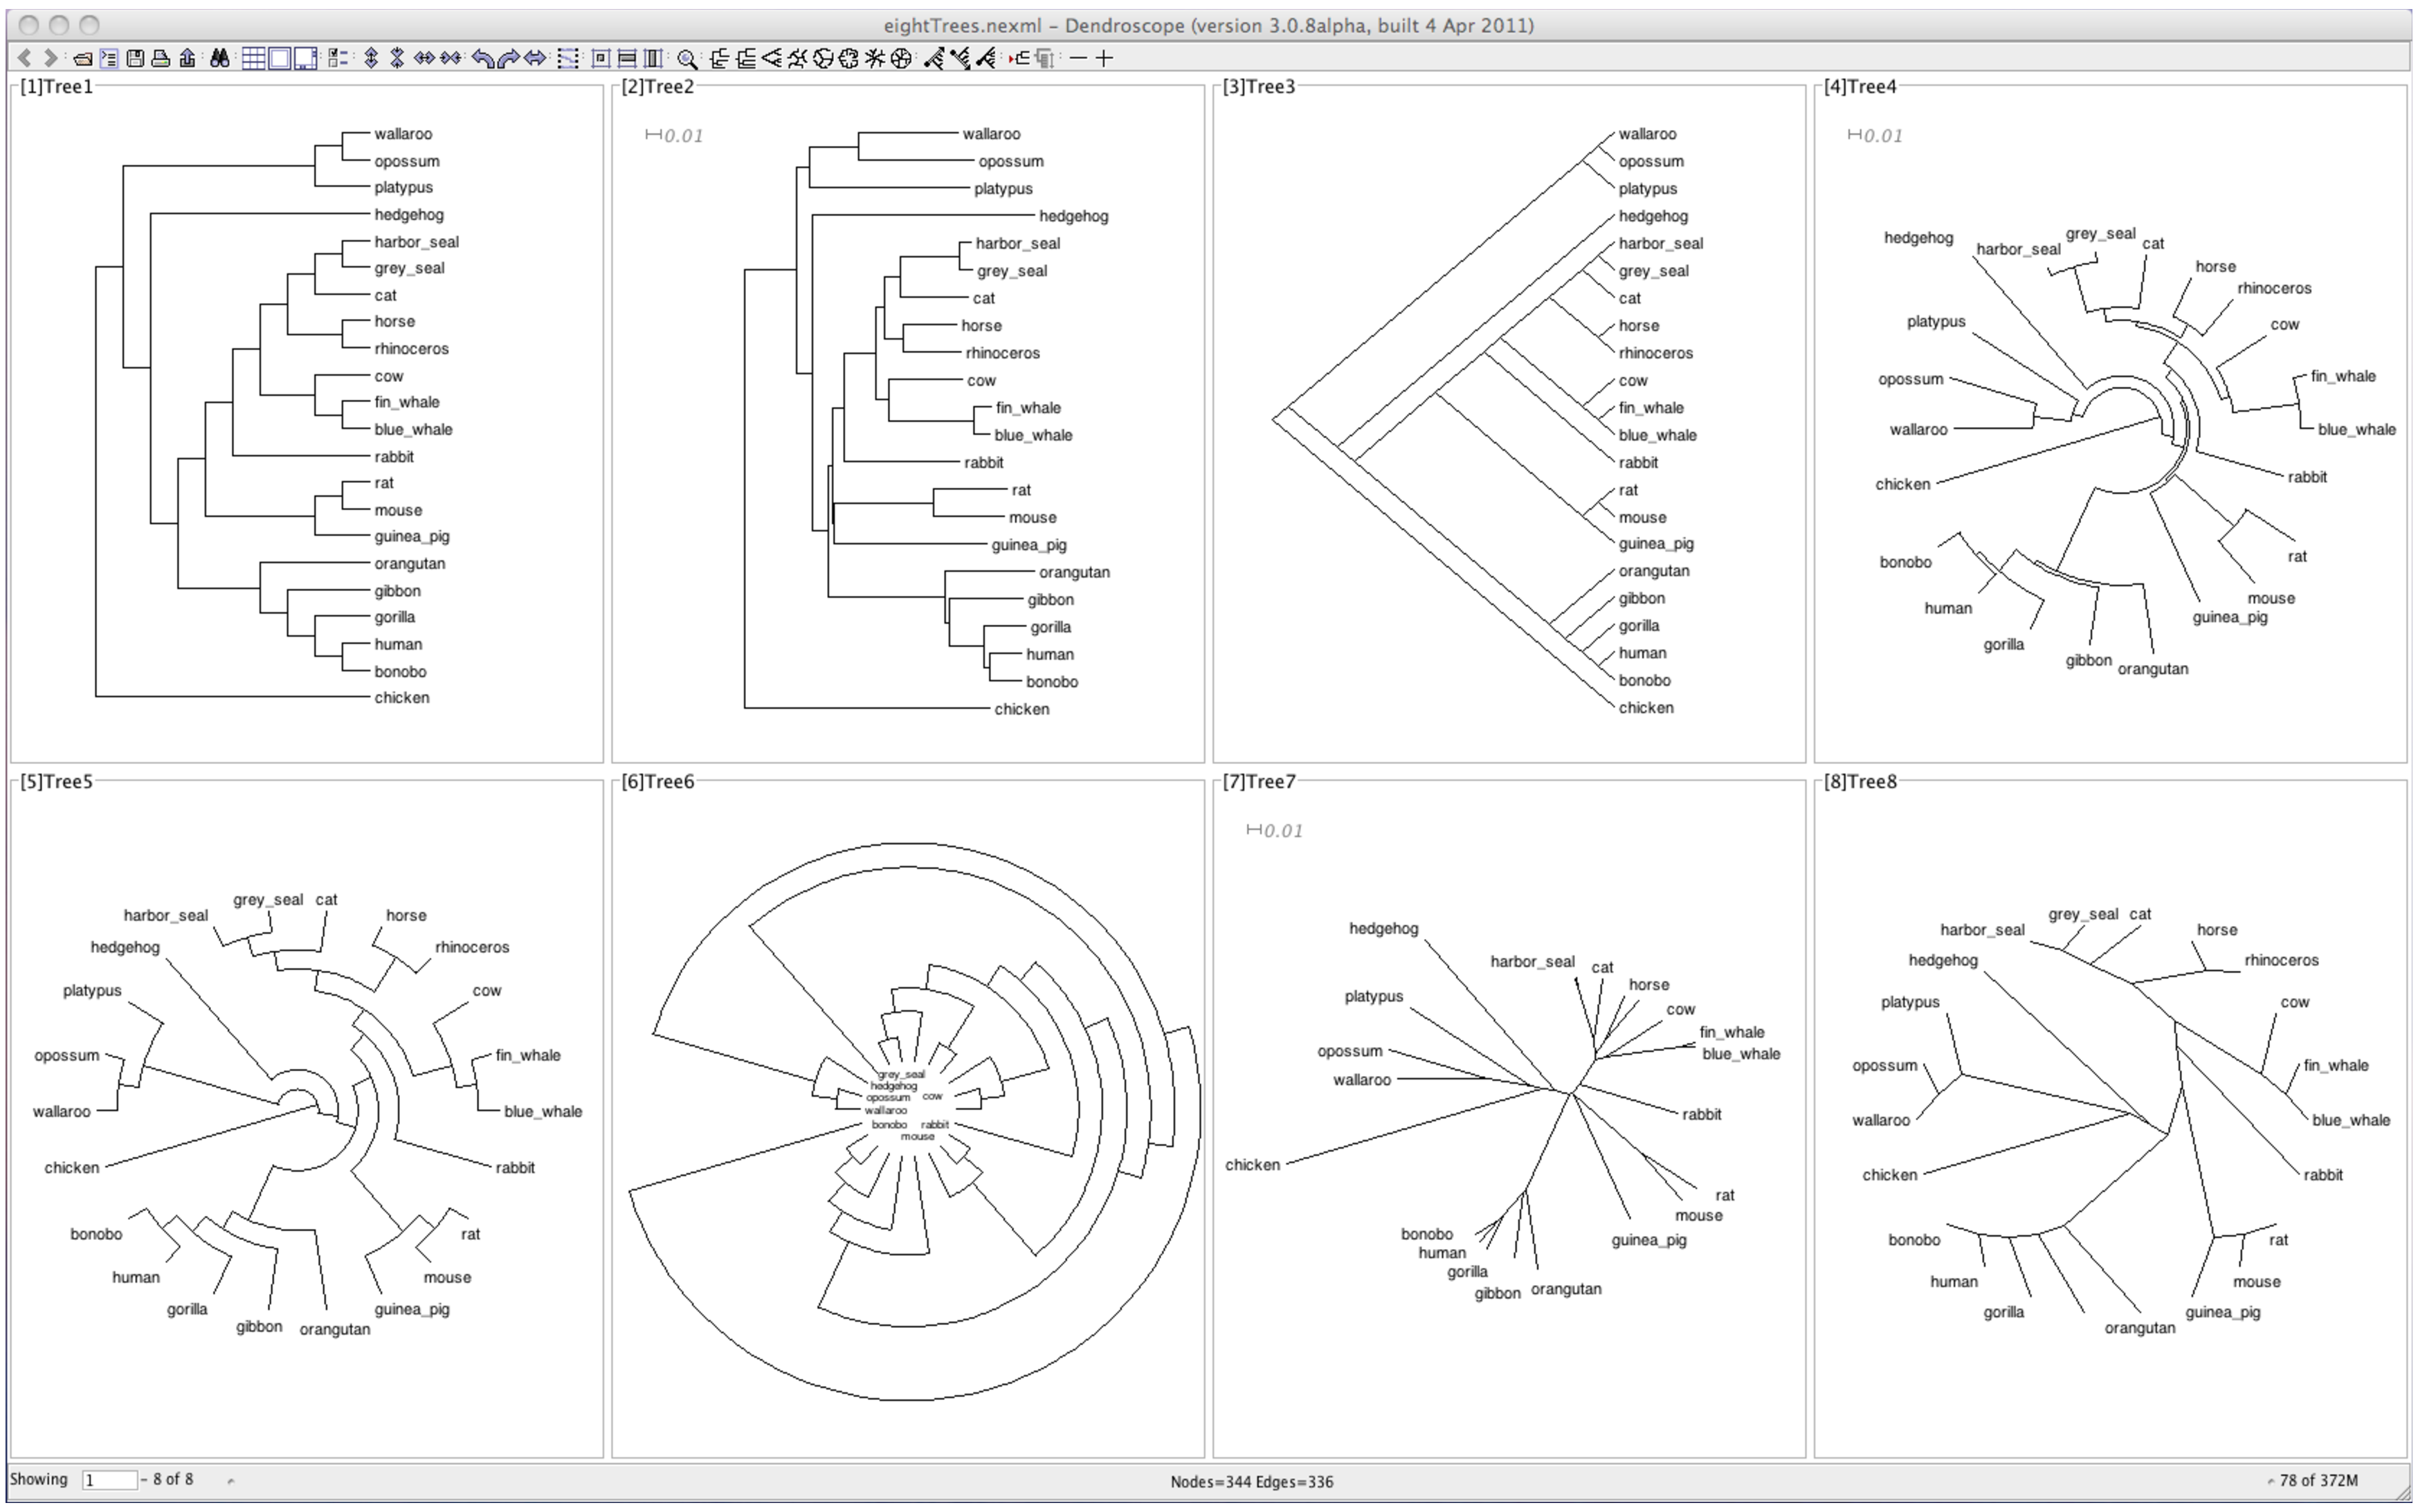
\includegraphics[width=1.0\textwidth]{./figs/eightTrees-2.pdf}
\end{center}
\caption{\small \sffamily Illustration of the eight views possible with \Dendroscope. Upper line: Rectangular Phylogram, Rectangular Cladogram, Slanted Cladogram, Circular Phylogram. Lower line: Circular Cladogram, Internal Circular Cladogram, Radial Phylogram, Radial Cladogram.}
\label{figure:7views}
\end{figure}

\mysubsection{Additional tree view features}

Figure  \ref{figure:Magnifier1} illustrates the action of the Magnifier on part of the NCBI taxonomy tree close to \textit{Homo sapiens}.

\begin{figure}[ht] % b floats figure to bottom, p floats to next page, h = here
\begin{center}

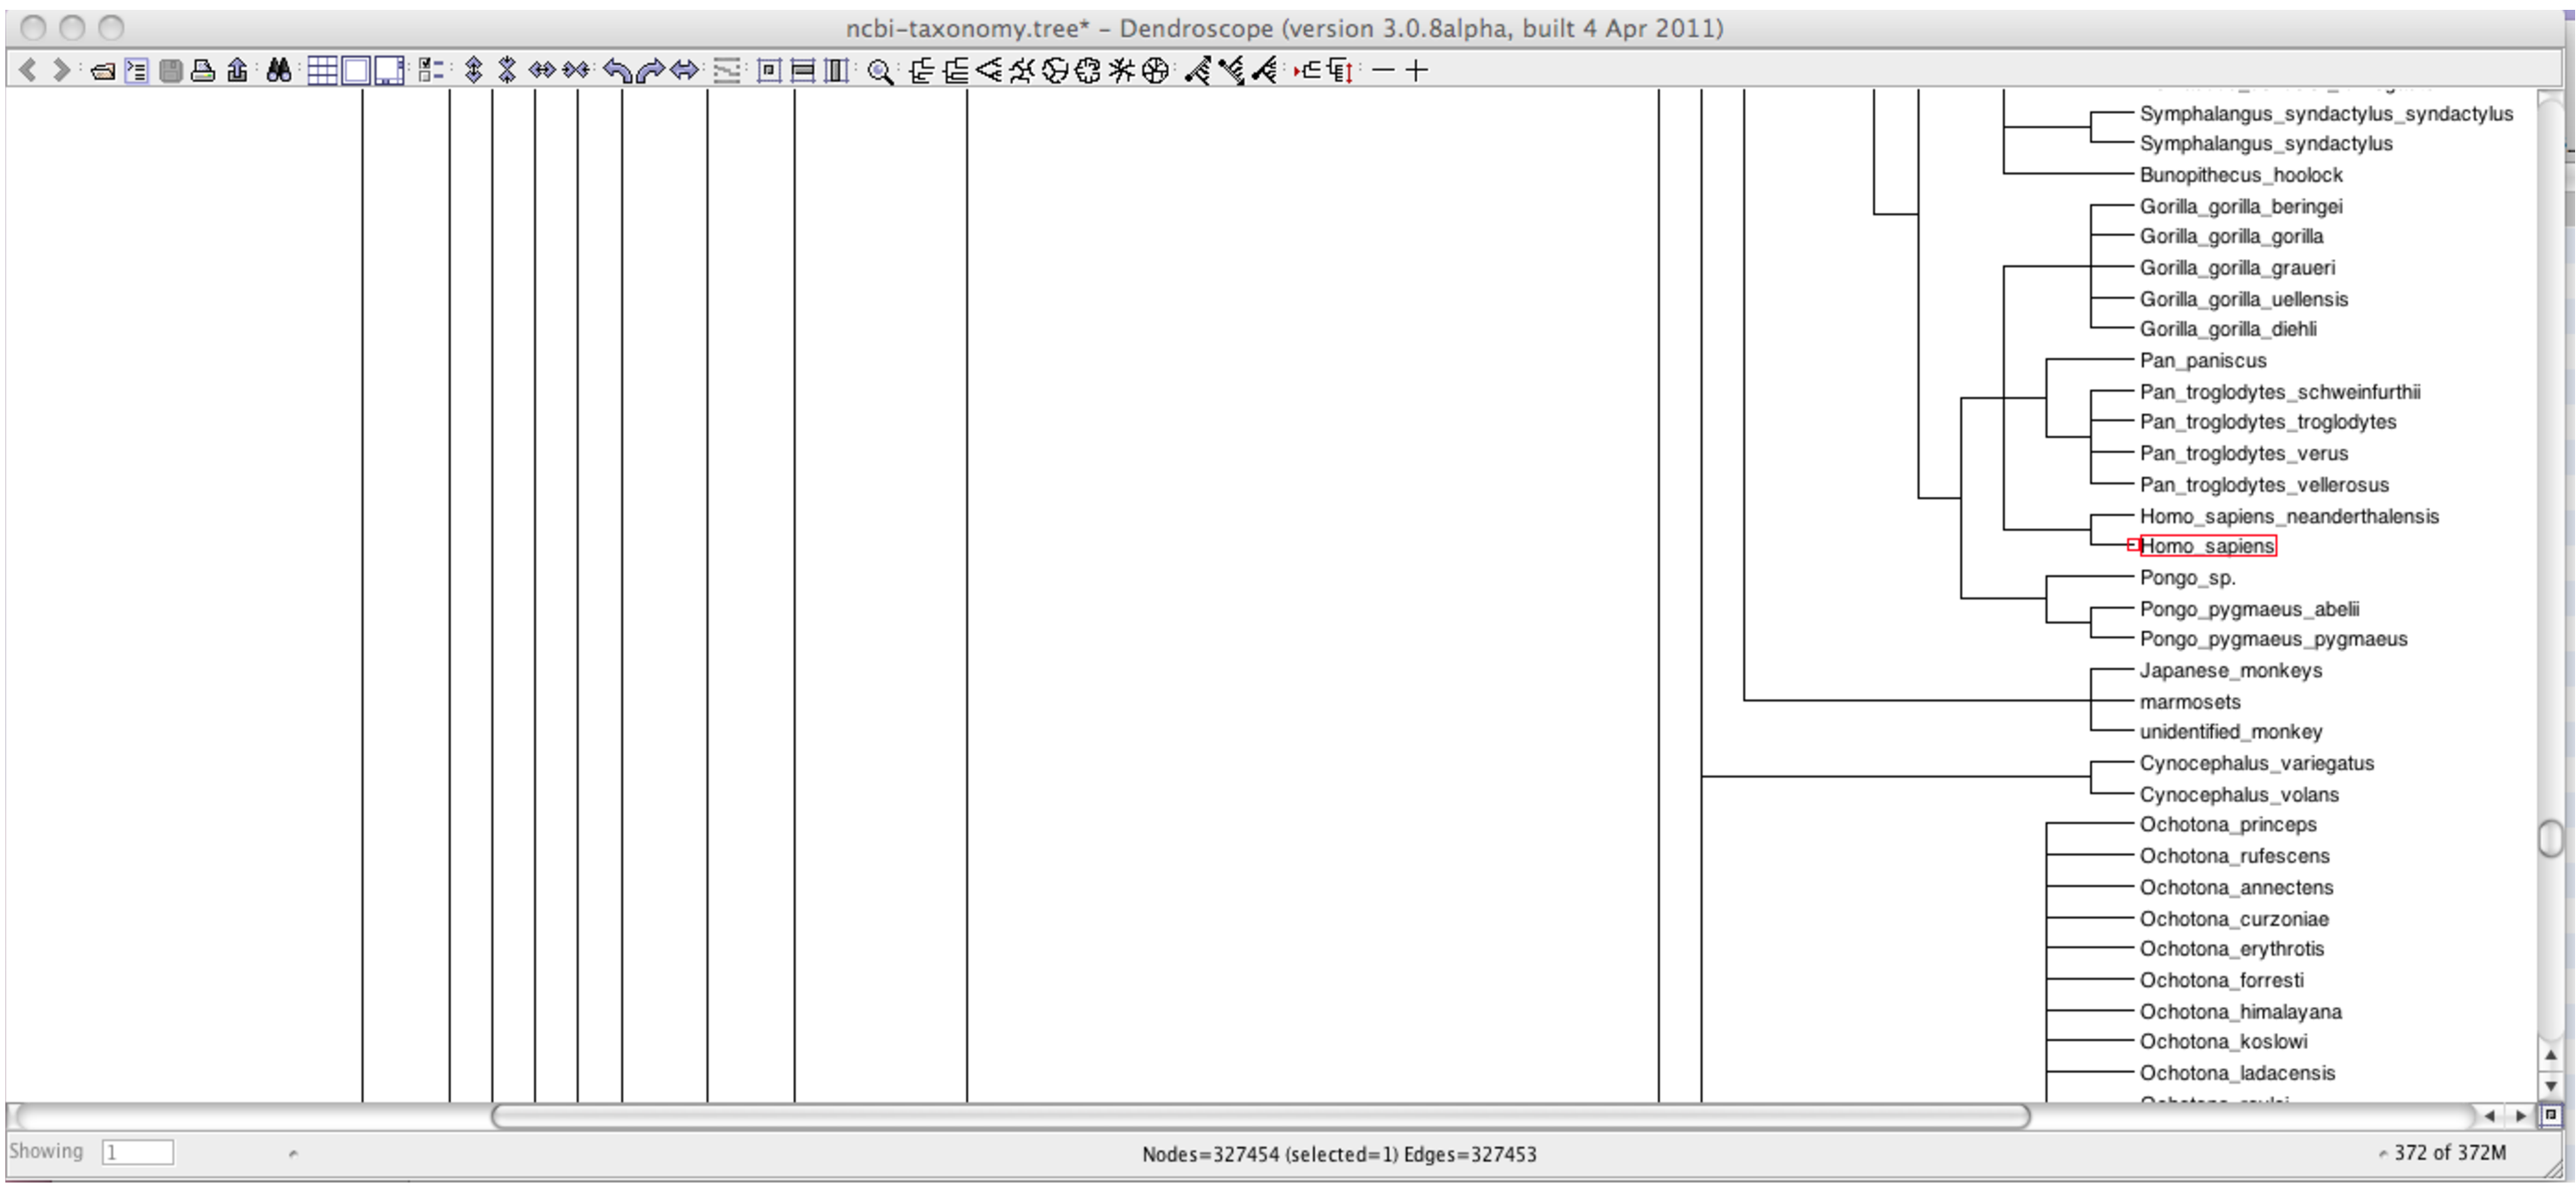
\includegraphics[width=0.85\textwidth]{./figs/ncbi-taxonomy.pdf}
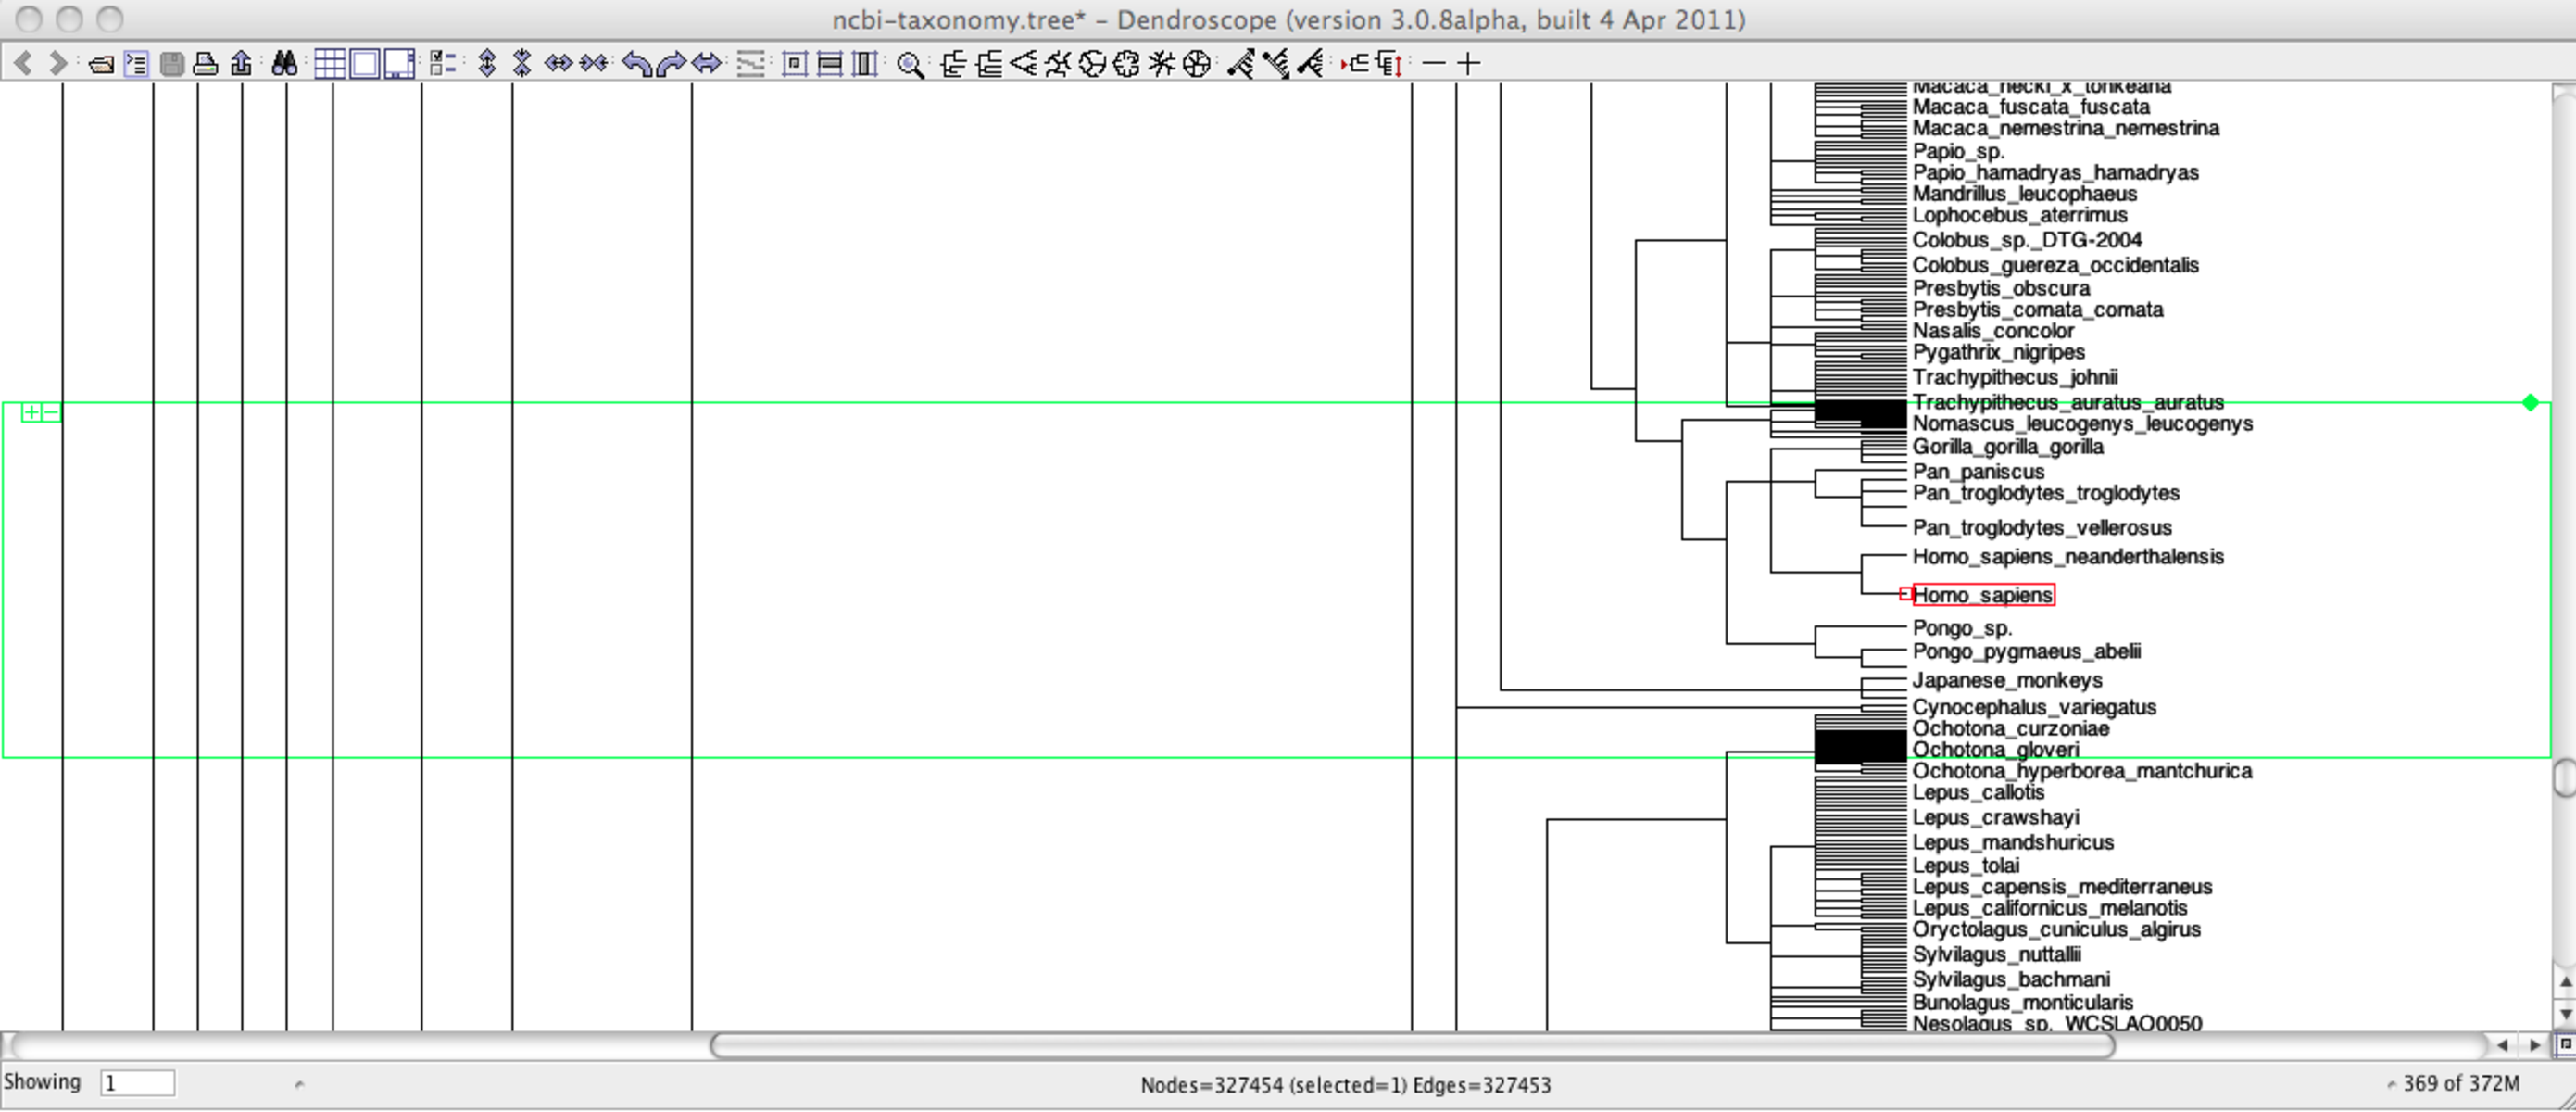
\includegraphics[width=0.85\textwidth]{./figs/ncbi-taxonomy3.pdf}

\end{center}
\caption{\small \sffamily Part of the NCBI taxonomy showing \textit{Homo sapiens} and his relatives without and with the magnifier turned on.}
\label{figure:Magnifier1}
\end{figure}


\mysubsection{Editing trees}

Figure \ref{figure:editedTree} demonstrates some of the editing possibilities present in Dendroscope.


\begin{figure}[ht] % b floats figure to bottom, p floats to next page, h = here
\begin{center}
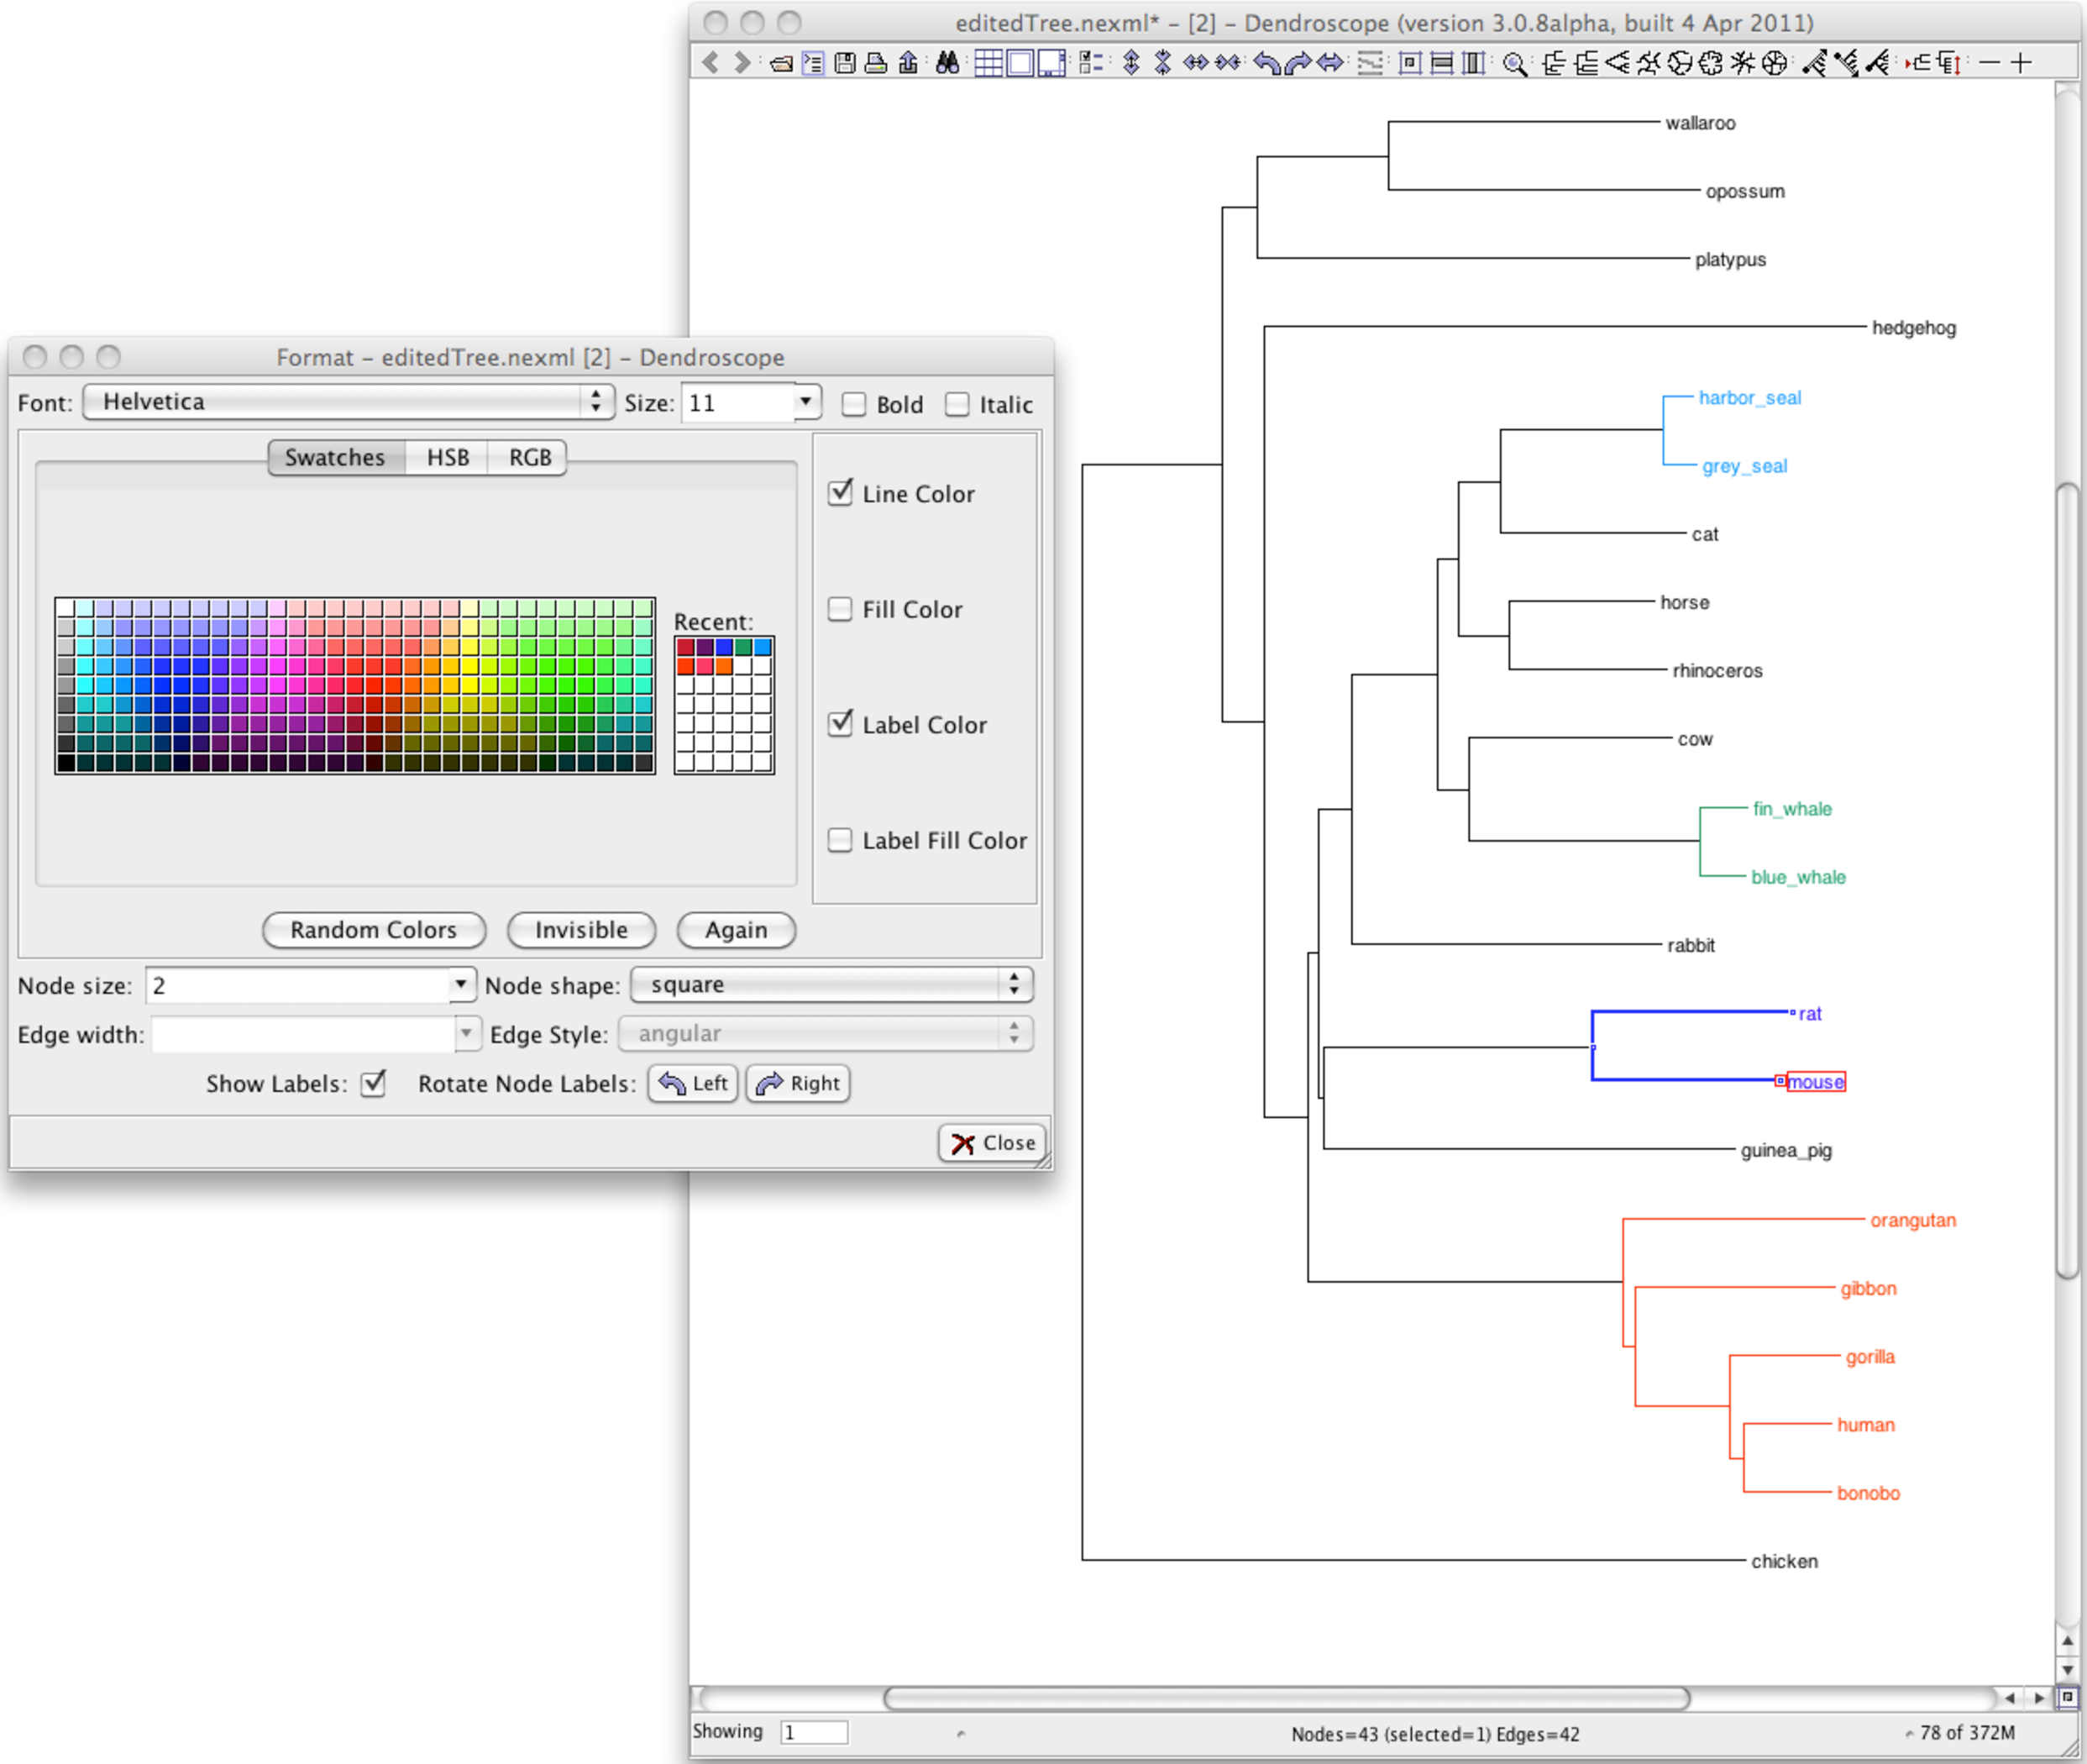
\includegraphics[width=0.9\textwidth]{./figs/editedTree.pdf}
\end{center}	
\caption{\small \sffamily All labels and tree substructures can be easily edited.}
\label{figure:editedTree}
\end{figure}


\mysubsection{Constructing rooted phylogenetic networks}


Figure \ref{figure:hybridNet} depicts two phylogenetic trees from the 
Poaceae dataset from the Grass Phylogeny Working Group \cite{gpwg2001} and the 4  hybrid networks computed from these trees by the method presented in \cite{Albrecht2012}.


\begin{figure}[ht] % b floats figure to bottom, p floats to next page, h = here
\begin{center}
\begin{tabular}{ccc}
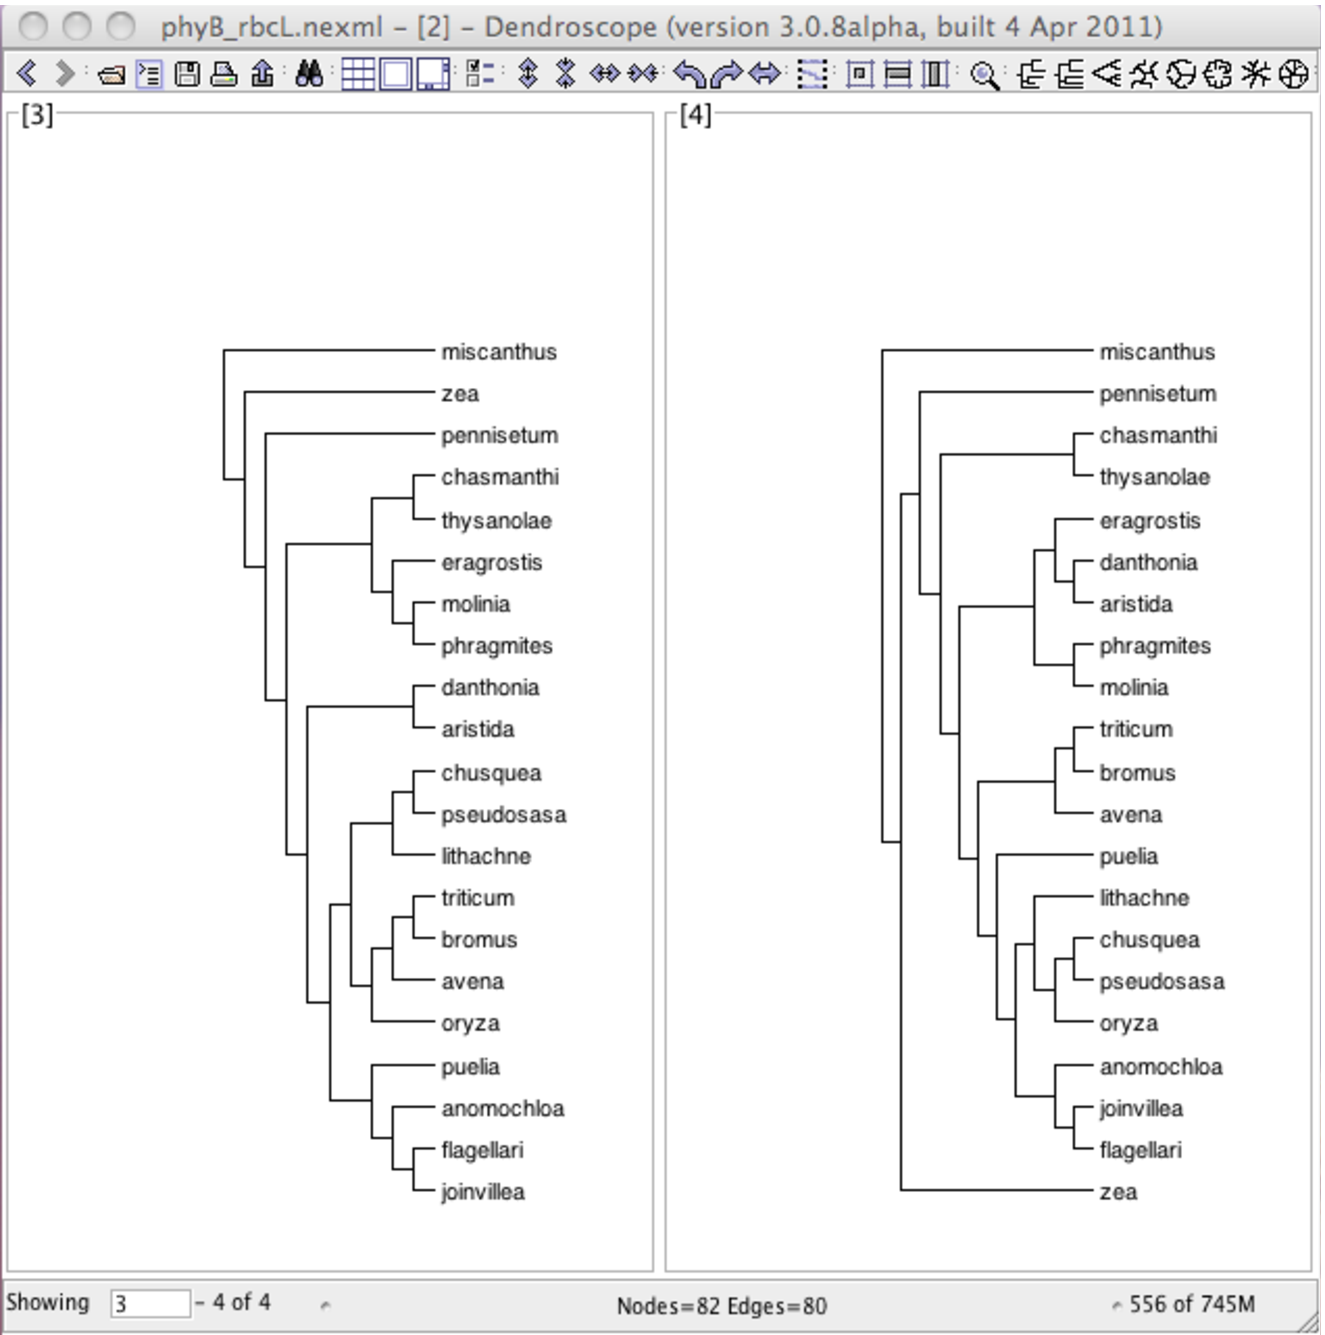
\includegraphics[width=0.42\textwidth]{./figs/phyB_rbcL.pdf}&
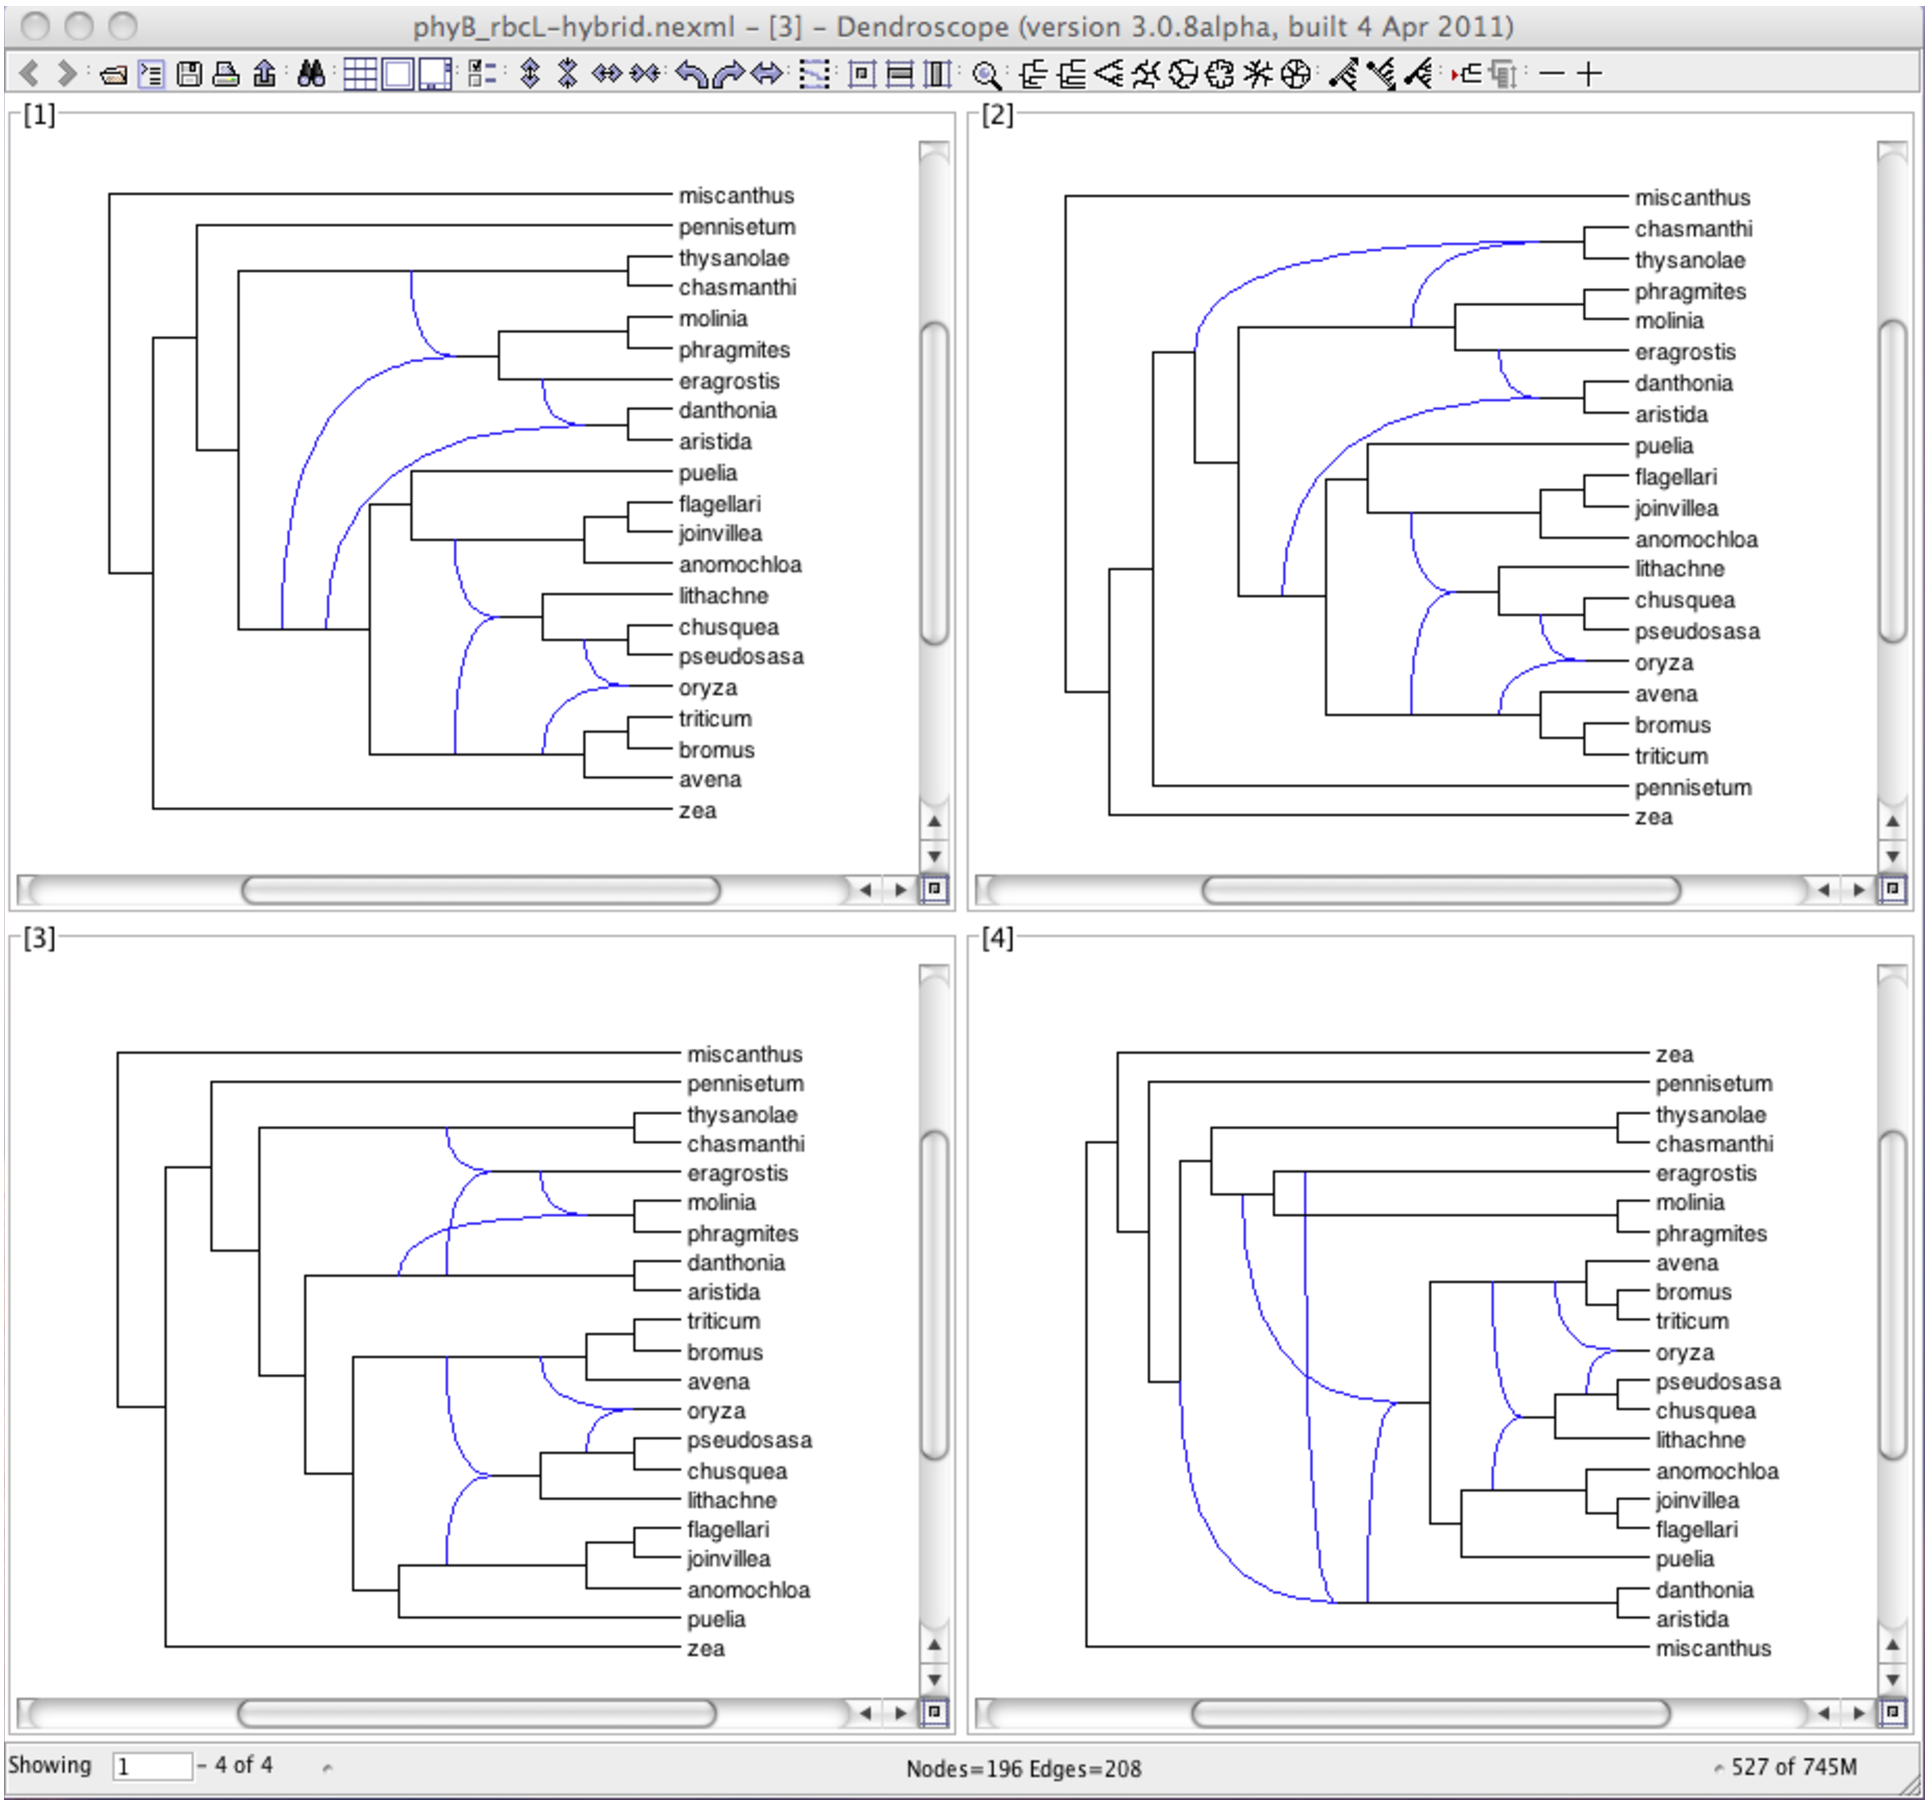
\includegraphics[width=0.45\textwidth]{./figs/phyB_rbcL-hybrid.pdf}\vspace{0.3cm}\\
(a)&(b)
\end{tabular}
\end{center}	
\caption{\small \sffamily 
(a) Two phylogenetic trees from the 
Poaceae dataset from the Grass Phylogeny Working Group \cite{gpwg2001}. The trees have been built from the loci 
{\em phytochrome B} (left) 
and {\em ribulose 1,5-biphosphate carboxylase/oxygenase, large subunit} (right) \cite{Schmidt2003}. (b) The 4  hybrid networks for the trees in (a) reconstructed  by the method presented in \cite{Albrecht2012}.
}
\label{figure:hybridNet}
\end{figure}

\mysubsection{Tanglegram}

Figure \ref{figure:tanglegram} shows a tanglegram between the first two networks in Figure \ref{figure:hybridNet}(b).

\begin{figure}[ht] % b floats figure to bottom, p floats to next page, h = here
\begin{center}
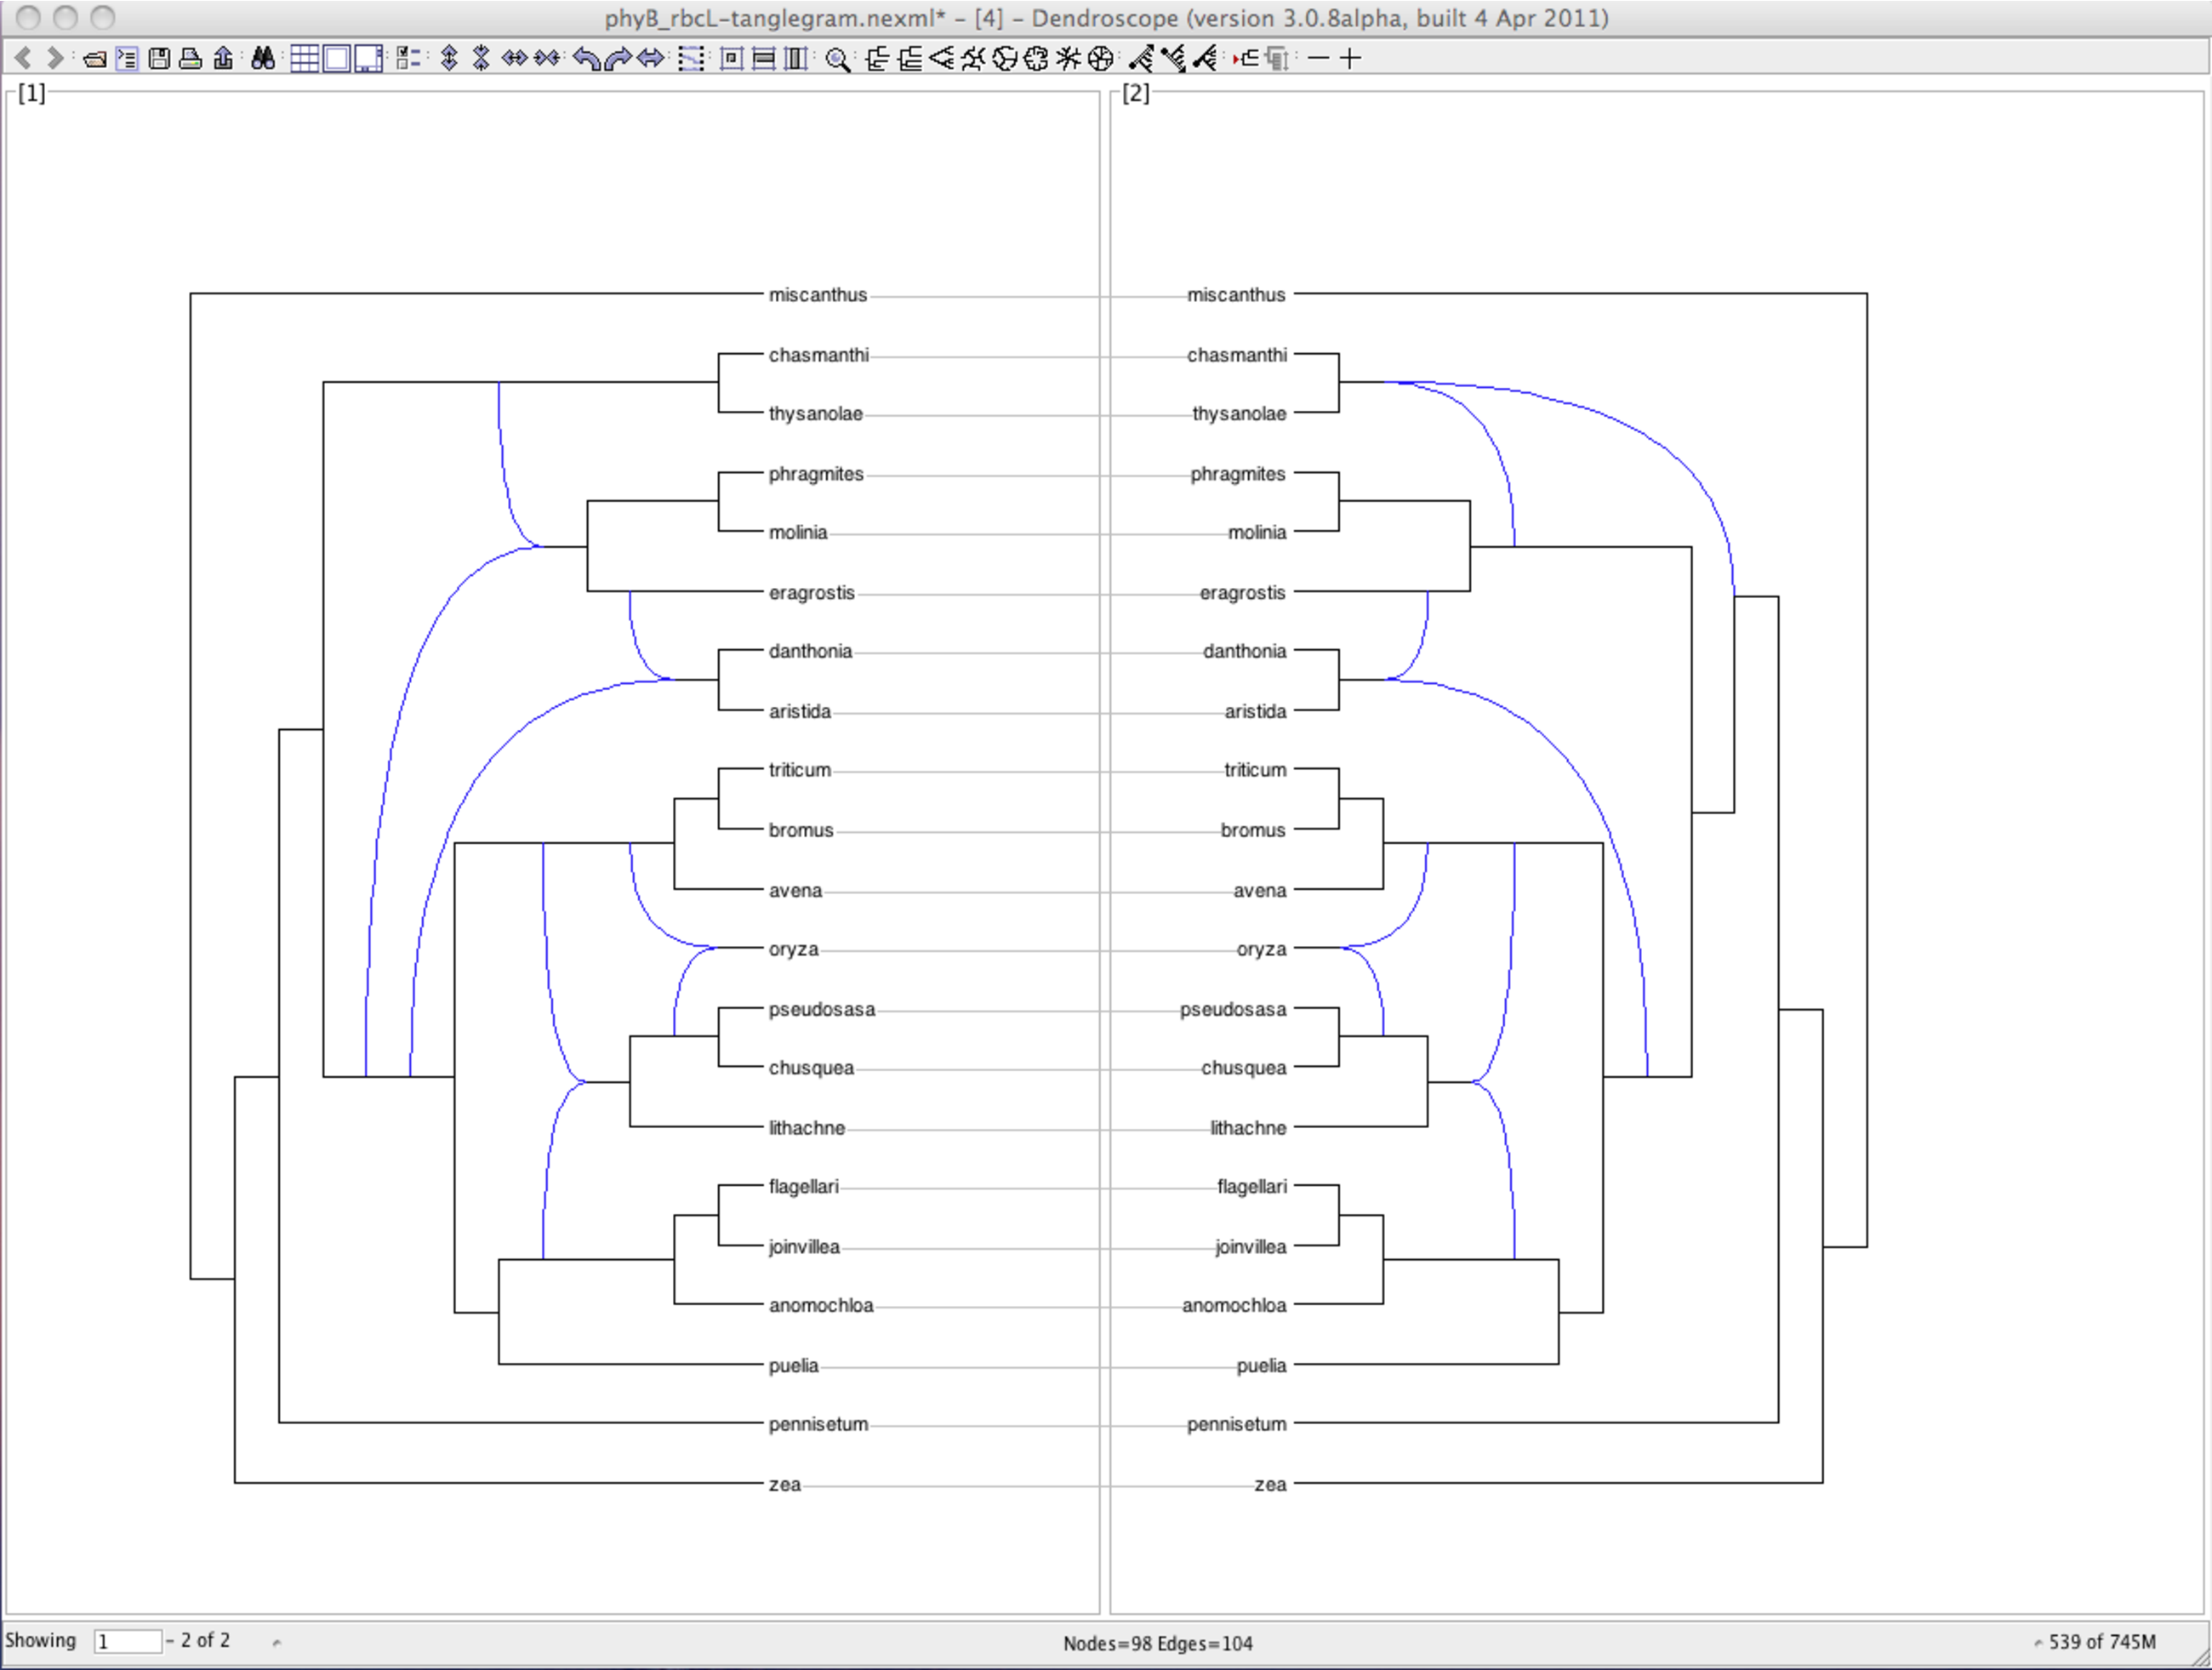
\includegraphics[width=0.9\textwidth]{./figs/phyB_rbcL-hybrid-tanglegram.pdf}
\end{center}	
\caption{\small \sffamily A tanglegram for two phylogenetic networks.}
\label{figure:tanglegram}
\end{figure}





%%%%%%%%%%%%%%%%%%%%%%%%%%%%%%%%%%%%%%%%%%%%%%%
\mysection{Acknowledgements}
%%%%%%%%%%%%%%%%%%%%%%%%%%%%%%%%%%%%%%%%%%%%%%%

This program includes  software developed  by the  Apache Software Foundation
(\url{http://www.apache.org/}), namely the \pconcept{Batik} library for
generating image files.
It also uses \pconcept{MRJAdapter}, a Java
package used to help construct user interfaces for the Apple Macintosh.
This program uses Daniel Huson's unpublished {\tt jloda} library, which is also
used by SplitsTree4 (\url{http://www.splitstree.org})\cite{SplitsTree98,HusonBryant2006}.


%%%%%%%%%%%%%%%%%%%%%%%%%%%%%%%%%%%%%%%%%%%%%%%
\bibliographystyle{plain}
\bibliography{compbio-2012.bib}

\printindex

\end{document}
